\documentclass[12pt,longbibliography]{article}
\usepackage[utf8]{inputenc}
\usepackage[T1]{fontenc}
\usepackage[catalan]{babel}
\usepackage[a4paper, margin=2.7cm]{geometry}

\usepackage{amsmath, amsthm, amsfonts, amssymb}
\newtheorem{thm}{Theorem}[section]
\newtheorem{cor}[thm]{Corollary}
\newtheorem{lem}[thm]{Lemma}
\newtheorem{prop}[thm]{Proposition}
\theoremstyle{definition}
\newtheorem{defn}[thm]{Definition}
\theoremstyle{remark}
\newtheorem{rem}[thm]{Remark}

\usepackage{mathrsfs} 
\usepackage[colorlinks=true,linkcolor=blue,citecolor=blue,urlcolor=blue,breaklinks]{hyperref}

\usepackage{bbm} 

\usepackage{hyperref}
\usepackage{graphicx}
\graphicspath{ {Imatges portada/} }

\title{Big Query}
\author{Anna Salazar}

\renewcommand{\contentsname}{Índex}
\renewcommand{\figurename}{Figura}
\renewcommand{\tablename}{Taula}

\begin{document}
\begin{titlepage}
\maketitle

\vspace{140mm}

\par
\raisebox{-.5\height}{
\includegraphics[width=6cm]{fme}}%
\hfill
\raisebox{-.5\height}{
\includegraphics[width=6cm]{UB}}%
\par

\end{titlepage}

\tableofcontents

\pagebreak

\pagenumbering{arabic}

\section{Què és BigQuery?}

BigQuery és un motor d’anàlisi de macrodades (Big Data) que permet executar consultes SQL al núvol sobre les dades emmagatzemades en aquest, sense importar el volum de les dades ni el tipus de consultes que es volen fer. El motor de consulta és capaç de treballar sobre terabytes de dades en qüestió de segons, i sobre petabytes en pocs minuts. Avui en dia, les empreses estan adoptant cada cop més la presa de decisions basades en dades i fomentant una cultura oberta en la qual les dades no estan aïllades dins dels departaments. BigQuery, en proporcionar els mitjans tecnològics per a promoure un canvi cultural cap a l’agilitat i l’obertura, realitza un paper molt important en l’augment del ritme de la innovació.

\vspace{2mm}

Treballar amb dades a BigQuery implica 3 aspectes principals: l’emmagatzemament, la incorporació de les dades i la consulta d’aquestes, Google s’encarrega de tota la resta. Com BigQuery és un servei totalment gestionat, no és necessari configurar ni instal·lar res en el nostre ordinador i, pel mateix motiu, no necessitem un administrador de la base de dades. Simplement, podem entrar en el nostre projecte de Google Cloud des del propi navegador i començar a analitzar.

\vspace{2mm}

Pel que fa a l’emmagatzemament, les dades es guarden en una taula estructurada, la qual cosa significa que es pot utilitzar SQL estàndard per a facilitar la consulta i l’anàlisi de dades. BigQuery és perfecta pel Big Data perquè gestiona tot aquest emmagatzemament i està proveïda d’operacions d’escalabilitat que funcionen de forma automàtica sense que l’usuari s’hagi d’involucrar,  per la qual cosa mai haurem de preocupar-nos per la grandària de les dades amb els quals treballem. Part de la consideració de disseny darrere de BigQuery és animar als usuaris a centrar-se en els coneixements en lloc de la infraestructura. Quan s’introdueixen les dades a BigQuery no és necessari pensar en els diferents tipus d’emmagatzemament, ni en els seus avantatges pel que fa a velocitat i cost; l’emmagatzemament està totalment gestionat.

\vspace{2mm}
\noindent
Per a més informació sobre BigQuery, es pot consultar la pàgina de \href{https://cloud.google.com/bigquery/docs/introduction}{Google Cloud}.

\subsection{Per què hauríem d'utilitzar BigQuery en lloc d'altres eines?}

Una de les característiques més rellevants que presenta BigQuery és que es tracta d'una plataforma sense servidor, és a dir, que els servidors s'executen en segon pla, sense l'intervenció de l'usuari. A més, presenta una alta disponibilitat, la qual cosa es tradueix en que no cal preocupar-se per la caiguda dels servidors, ja que la plataforma s'encarrega d'això. Per últim, BigQuery també té propietats d'escalabilitat automàtica que fan possible gestionar fins a petabytes de dades. Aquestes característiques no estan disponibles a la majoria de plataformes d'emmagatzament de dades tradicionals, i fan destacar BigQuery entre moltes.

\vspace{2mm}

Com en molts altres magatzems de dades, BigQuery és capaç de treballar amb moltes fonts de dades diferents. Podem pujar les dades des del nostre propi sistema d'arxius, de Google Cloud Storage, de Google Drive i de moltes fonts més. Després de fer-ho, es poden consultar aquestes dades utilitzant SQL estàndard o SQL heretat, el rendiment en qualsevol cas és excel·lent. Els resultats de les consultes solen emmagatzemar-se en la memòria cau durant 24 hores, de manera que les següents execucions d'aquesta consulta només hauran d'obtenir les dades de la memòria cau en lloc de fer-ho del disc. 


\pagebreak

\section{Creació i treball amb conjunts de dades i taules}

\subsection{Configuració de la Plataforma de Google Cloud (GCP)}

\graphicspath{ {BigQuery/Imatges tutorial/} }

Per utilitzar aquesta eina d’anàlisi només ens caldrà crear un compte a Google Cloud i treballar a la zona de proves que ofereix Google per operar de forma gratuïta.
Per fer servir la zona de proves (\textit{Sandbox}) seguirem els passos següents: 

\vspace{2mm}

1. En primer lloc, ens dirigim a la interfície d’usuari (UI) de \href{https://console.cloud.google.com}{BigQuery}. Des d'aquesta interfície es poden realitzar la majoria de les operacions.

\vspace{2mm}

2. Accedim al nostre compte de Google o creem un nou compte si encara no en tenim cap. Si és el primer cop que iniciem sessió a Google Cloud, haurem de marcar el país on som i acceptar les condicions de servei.

\vspace{2mm}

3. Un cop dins, podem veure com és l'espai de treball SQL. Hi ha una secció de l'Explorador a l'esquerra que ens permet navegar en projectes, conjunts de dades i taules. Per tal de fer servir la zona de proves, haurem de crear un projecte.

Introdueix un nom al teu projecte i fes clic a Create. En el nostre cas, hem anomenat el projecte \verb|el_meu_projecte| (Figura ~\ref{fig:bq1}), i treballarem sobre aquest per il·lustrar el funcionament de la plataforma.

\vspace{2mm}
\begin{figure}[h!]
\par
\raisebox{-.5\height}{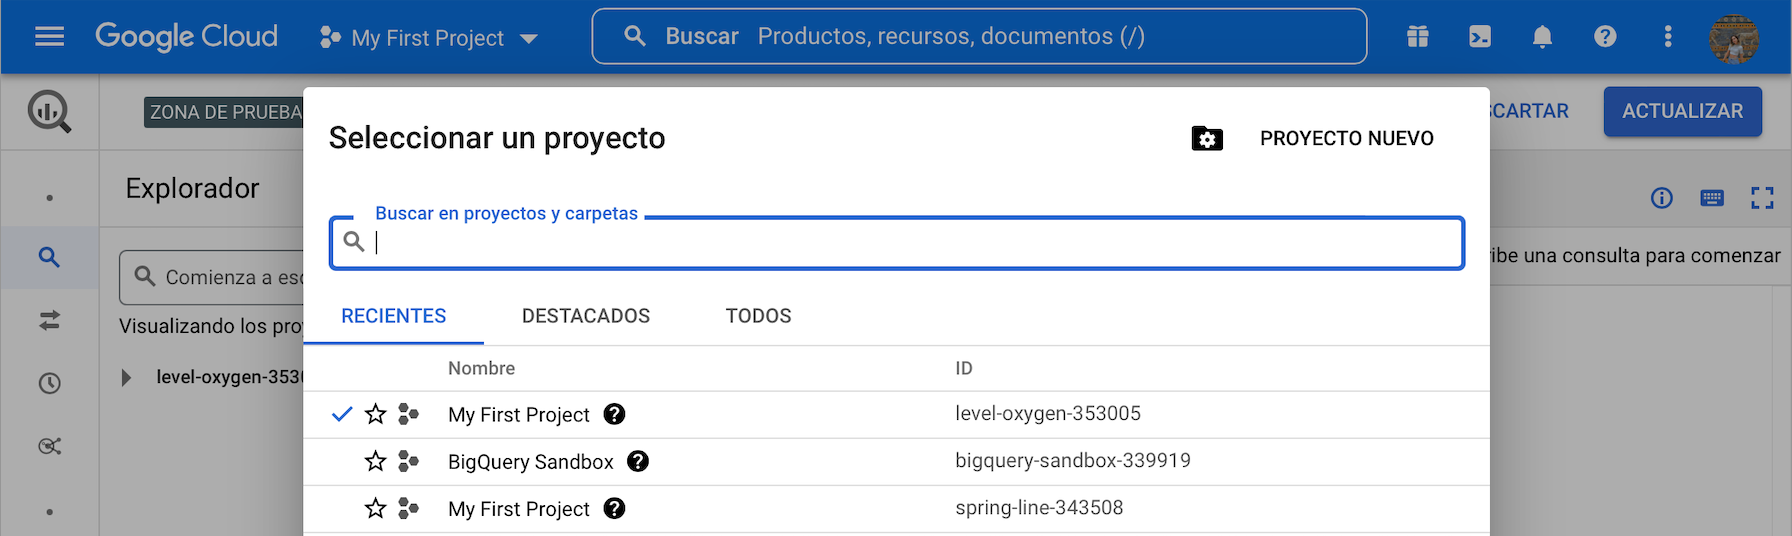
\includegraphics[width=7.25cm]{bq1}}%
\hfill
\raisebox{-.5\height}{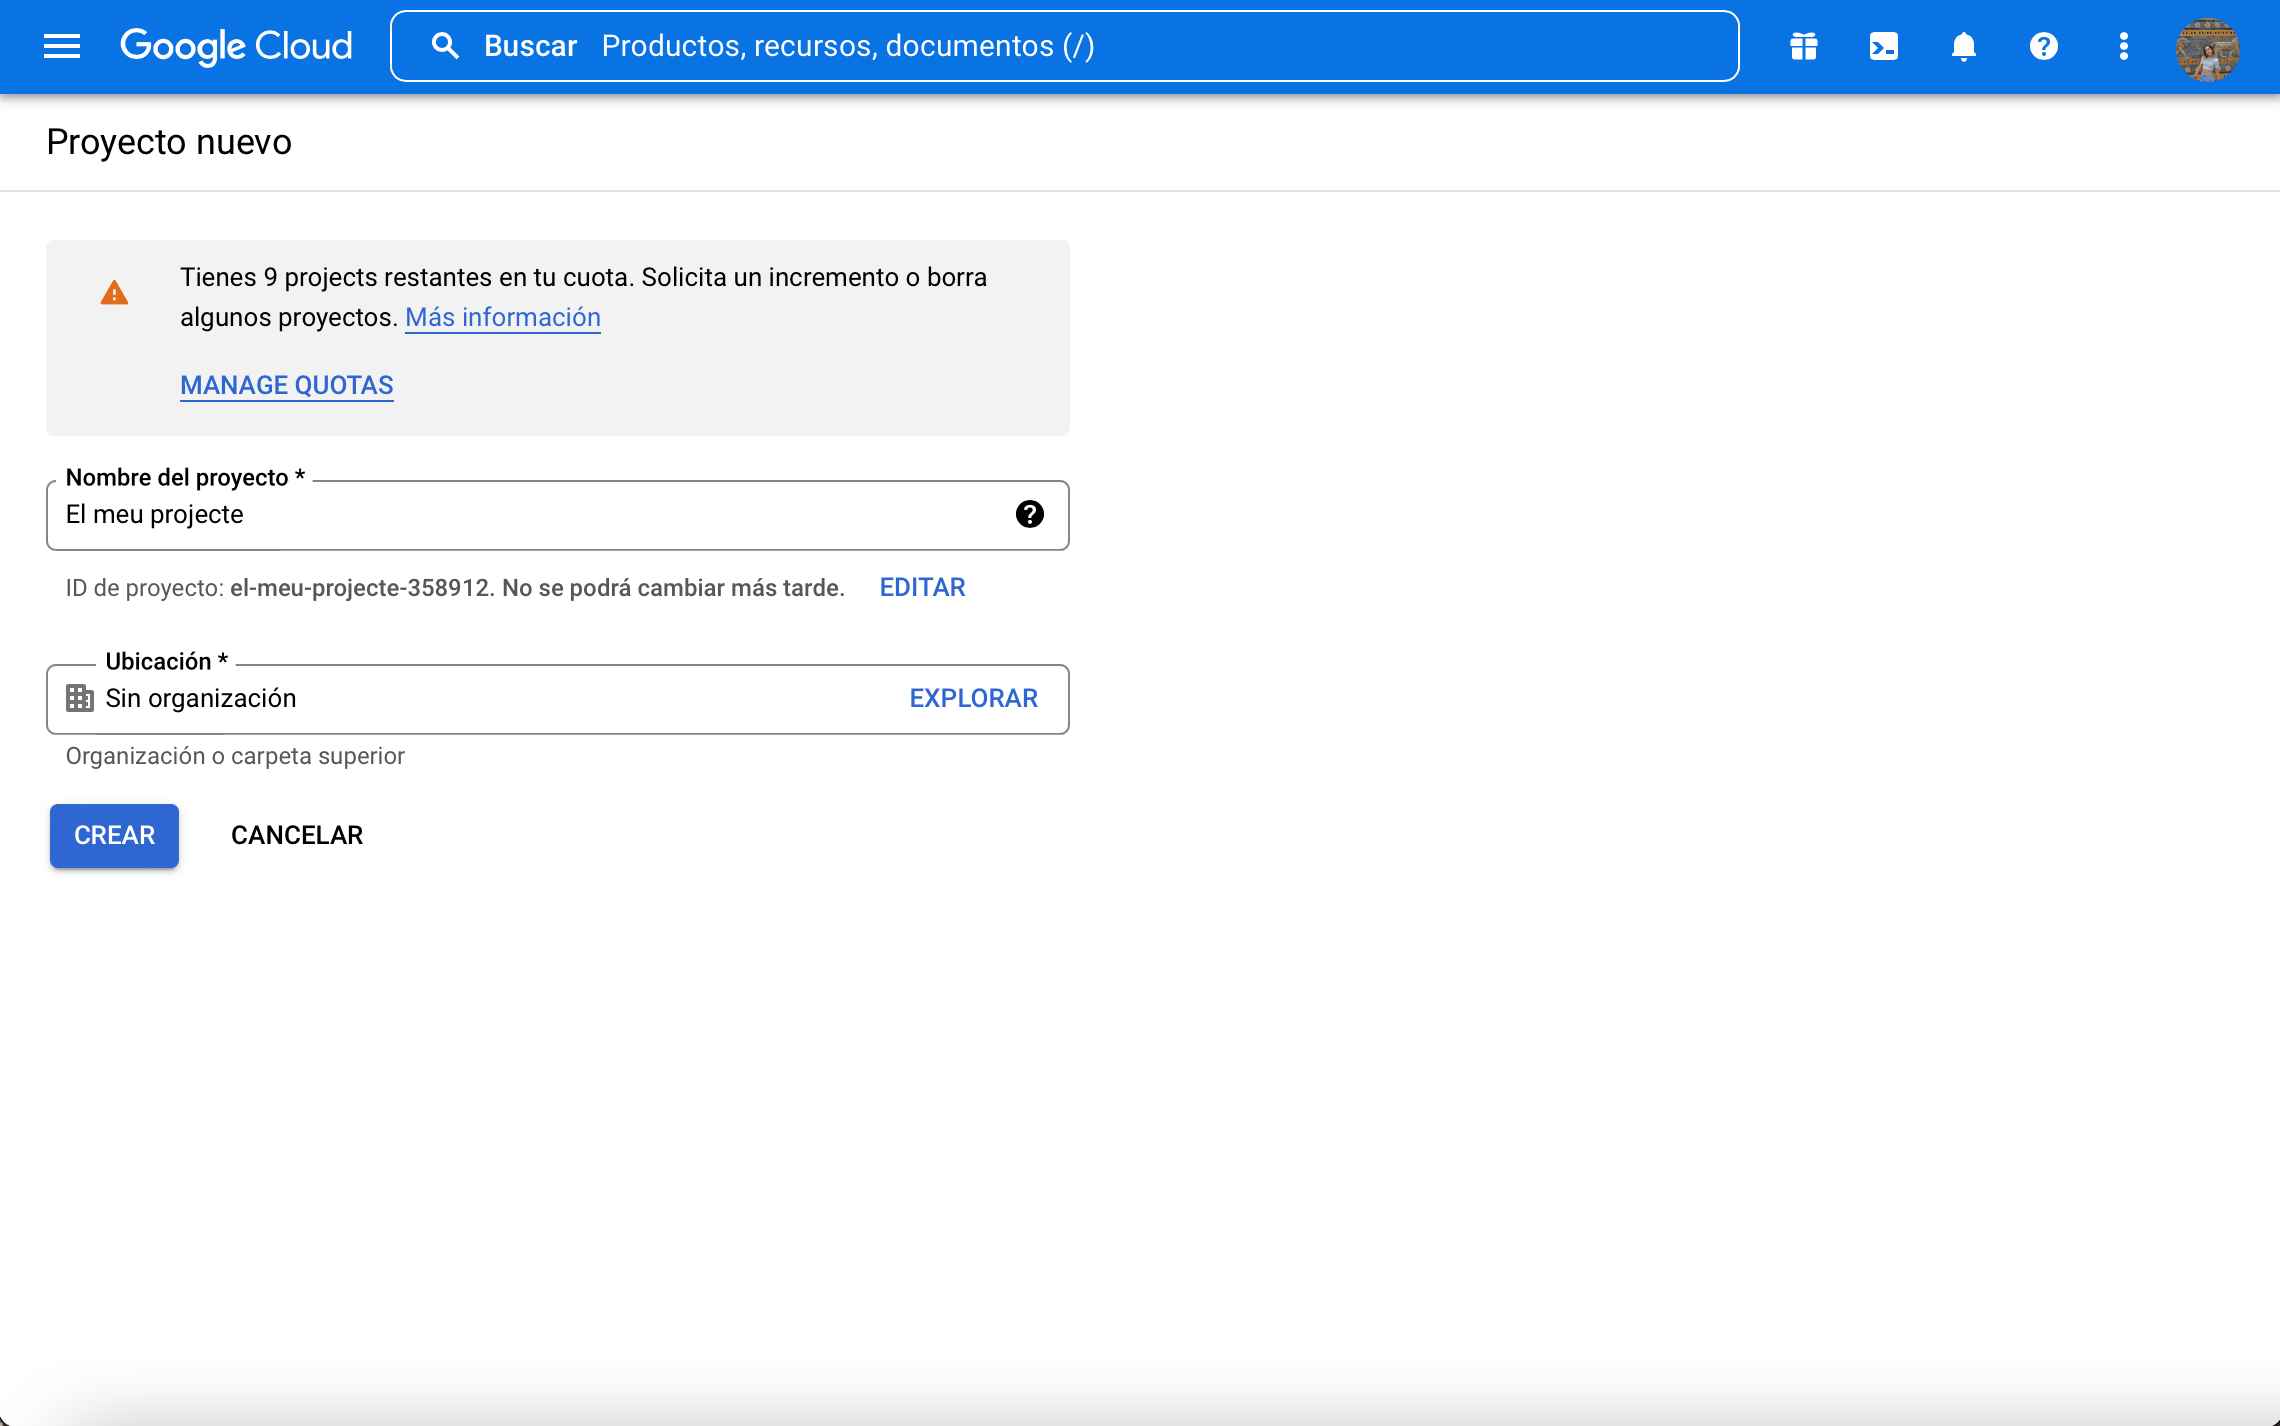
\includegraphics[width=7.25cm]{bq2}}%
\par
\caption{Creació d'un projecte}
\label{fig:bq1}
\end{figure}
\vspace{2mm}

4. Un cop creat el projecte, el navegador ens redirigigeix a la interfície web de BigQuery.

\vspace{2mm}

5. Ara ja podrem carregar o consultar dades en el nostre projecte sense cap compte de facturació adjunta.

\subsubsection{Limitacions}

Això no obstant, per a l’ús de la zona de proves gratuïta que ofereix Google, haurem de tenir en compte un seguit de limitacions.

\vspace{2mm}

En primer lloc, ens trobem amb un màxim de 10 Gb d’emmagatzemament i 10 Tb de consulta al mes. Al llarg d’aquest projecte no utilitzarem un volum de dades més gran ni sobrepassarem el límit d’espai de consulta, però s’han de tenir en compte aquestes limitacions si l’objectiu és treballar amb el format gratuït.

\vspace{2mm}

A més, ens trobem que tots els conjunts de dades tenen el temps de caducitat de la taula per defecte establerta en 60 dies. Per tant, totes les taules, vistes o particions de les taules caducaran automàticament passats els 60 dies.

\vspace{2mm}

Una altra característica destacable és que els projectes de la zona de proves no són compatibles amb:

- La transmissió de dades

- Sentència de llenguatge de manipulació de dades (DML)

- Servei de transferència de dades de BigQuery

\subsection{Creació d'un conjunt de dades}

Ara que ja coneixem les limitacions de la plataforma i disposem d'un projecte en el que crear un conjunt de dades, ha arribat el moment de crear un nou conjunt de dades dins d'aquest projecte. Es pot pensar en un conjunt de dades a BigQuery com una agrupació lògica de taules. Alhora, diferents cojunts de dades s'integren en un mateix projecte. 

\vspace{2mm}

Per a crear-ne un, només s'ha de desplegar el menú i triar l'opció de crear un nou conjunt de dades. Tot seguit hi ha diversos detalls per al conjunt de dades que es poden establir. En primer lloc, hi ha l'opció de canviar el projecte que l'encabirà. Això farà que aparegui un navegador on es podrà especificar el projecte. Una altra possibilitat serà escollir la ubicació de les dades. Això determina on s'aprovisionaran els recursos subjacents, com la computació i l'emmagatzematge, per al servei BigQuery. Les consideracions a l'hora de triar una ubicació inclouran el rendiment per als usuaris finals, l'alta disponibilitat i també qualsevol restricció d'auditoria o compliment. I, per últim, es pot establir un temps d'expiració per defecte per a les taules dins d'un conjunt de dades.

\vspace{2mm}
\begin{figure}[h!]
\par
\raisebox{-.5\height}{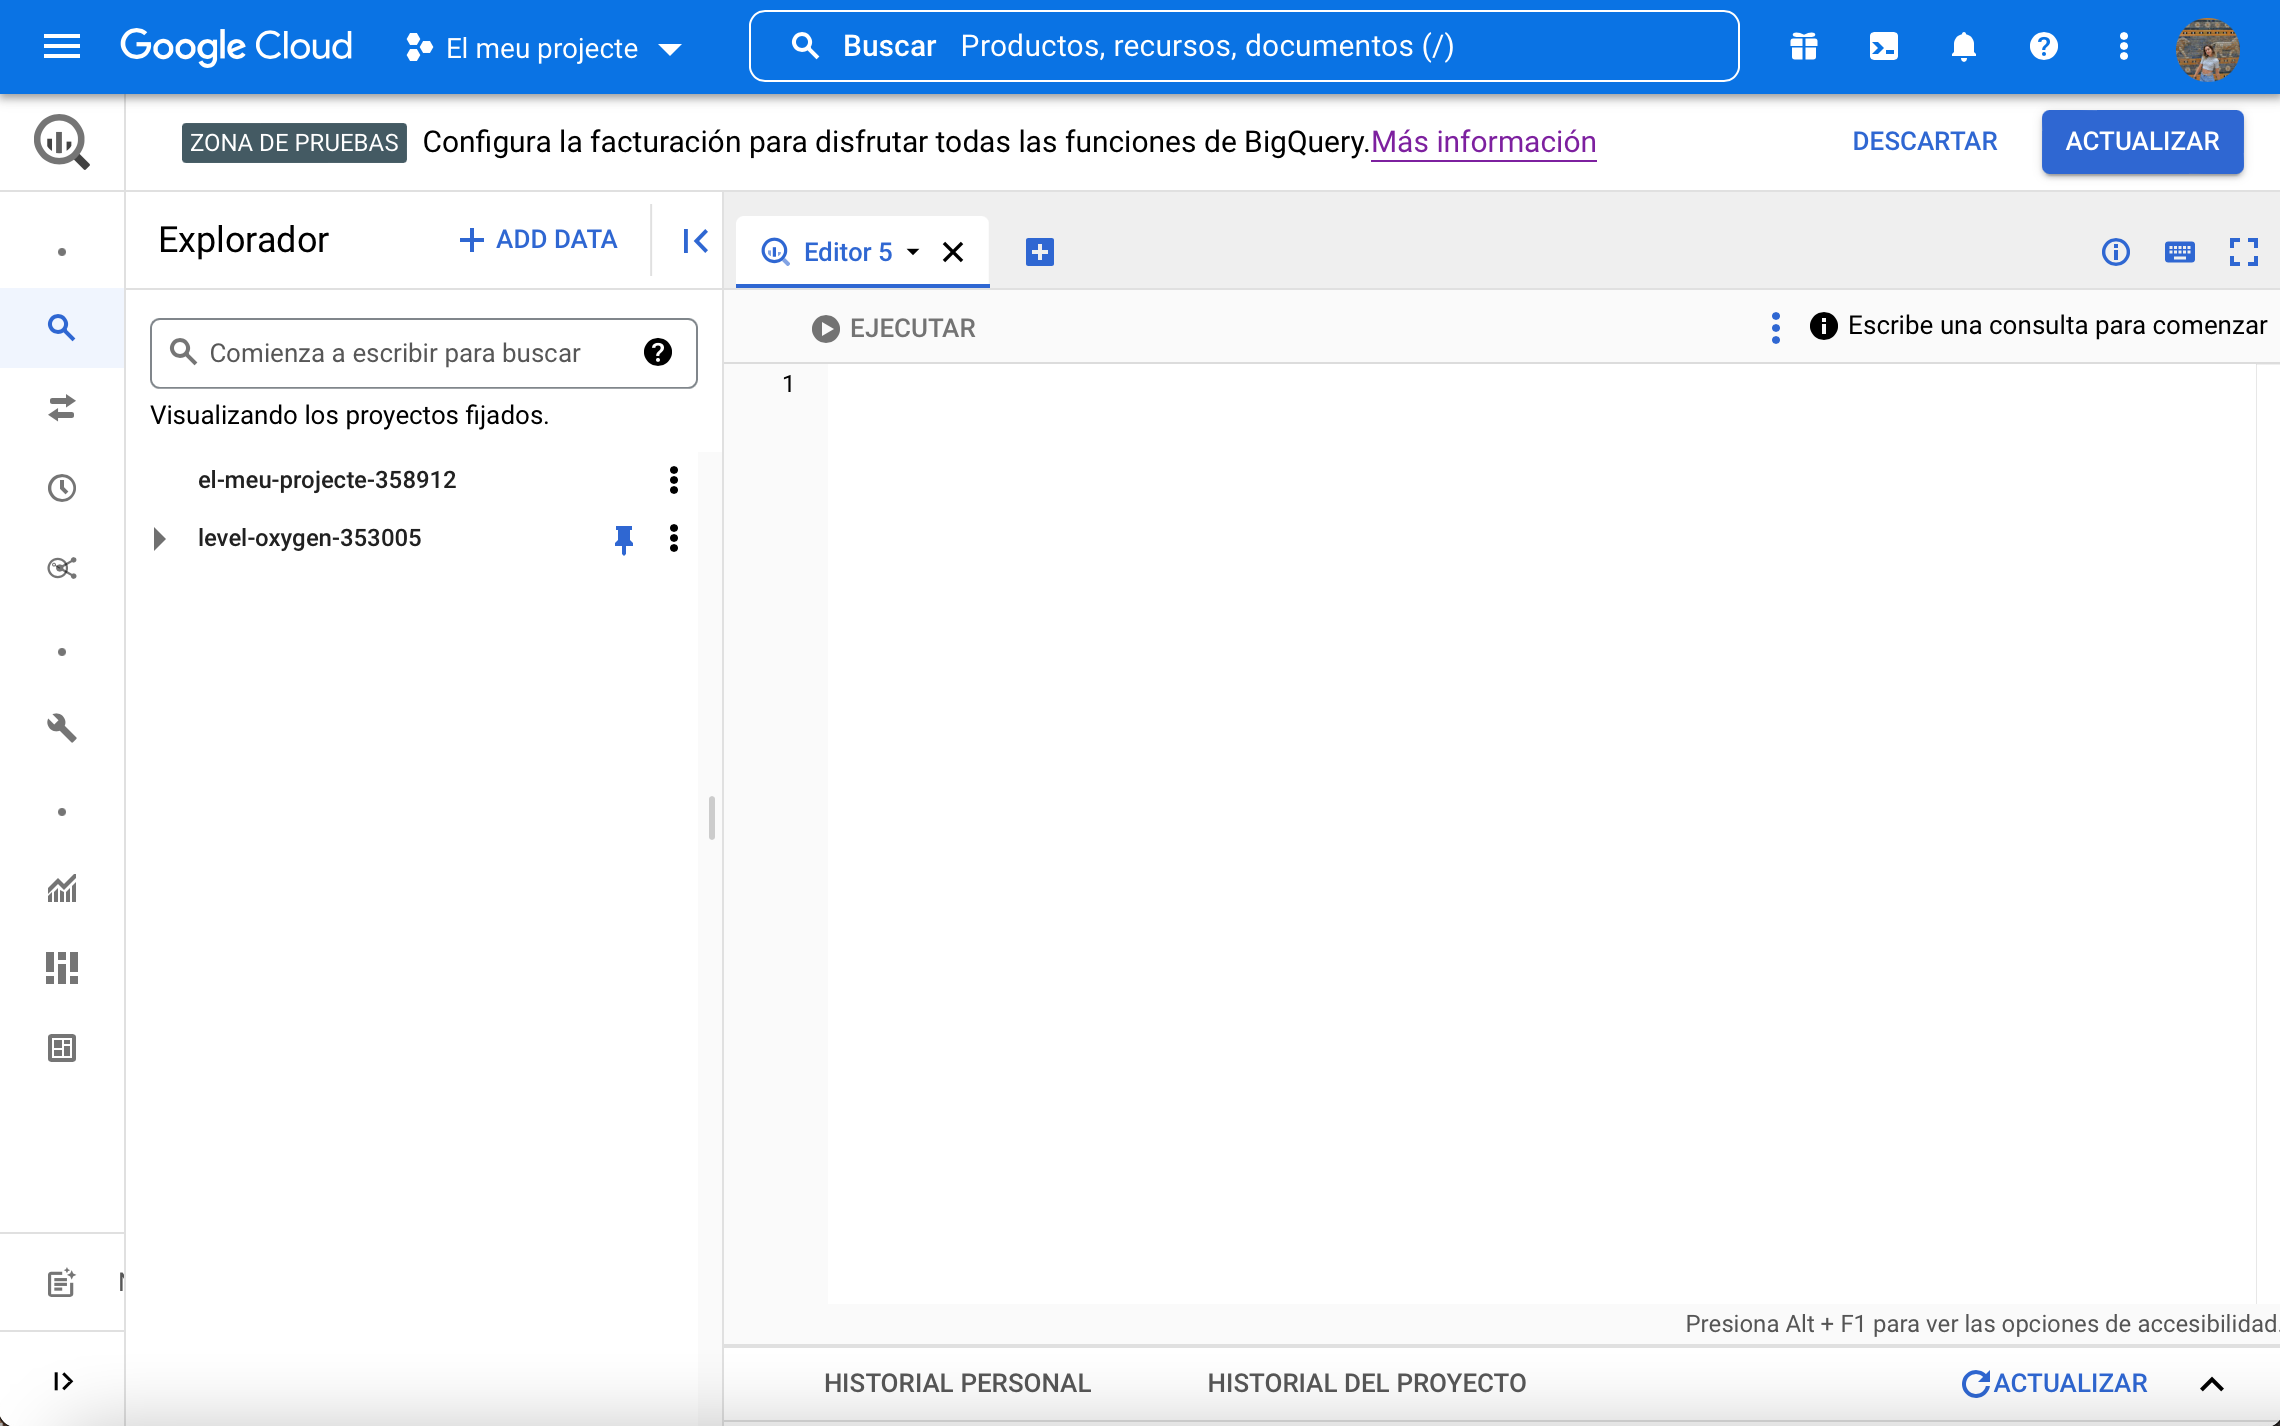
\includegraphics[width=7.25cm]{bq3}}%
\hfill
\raisebox{-.5\height}{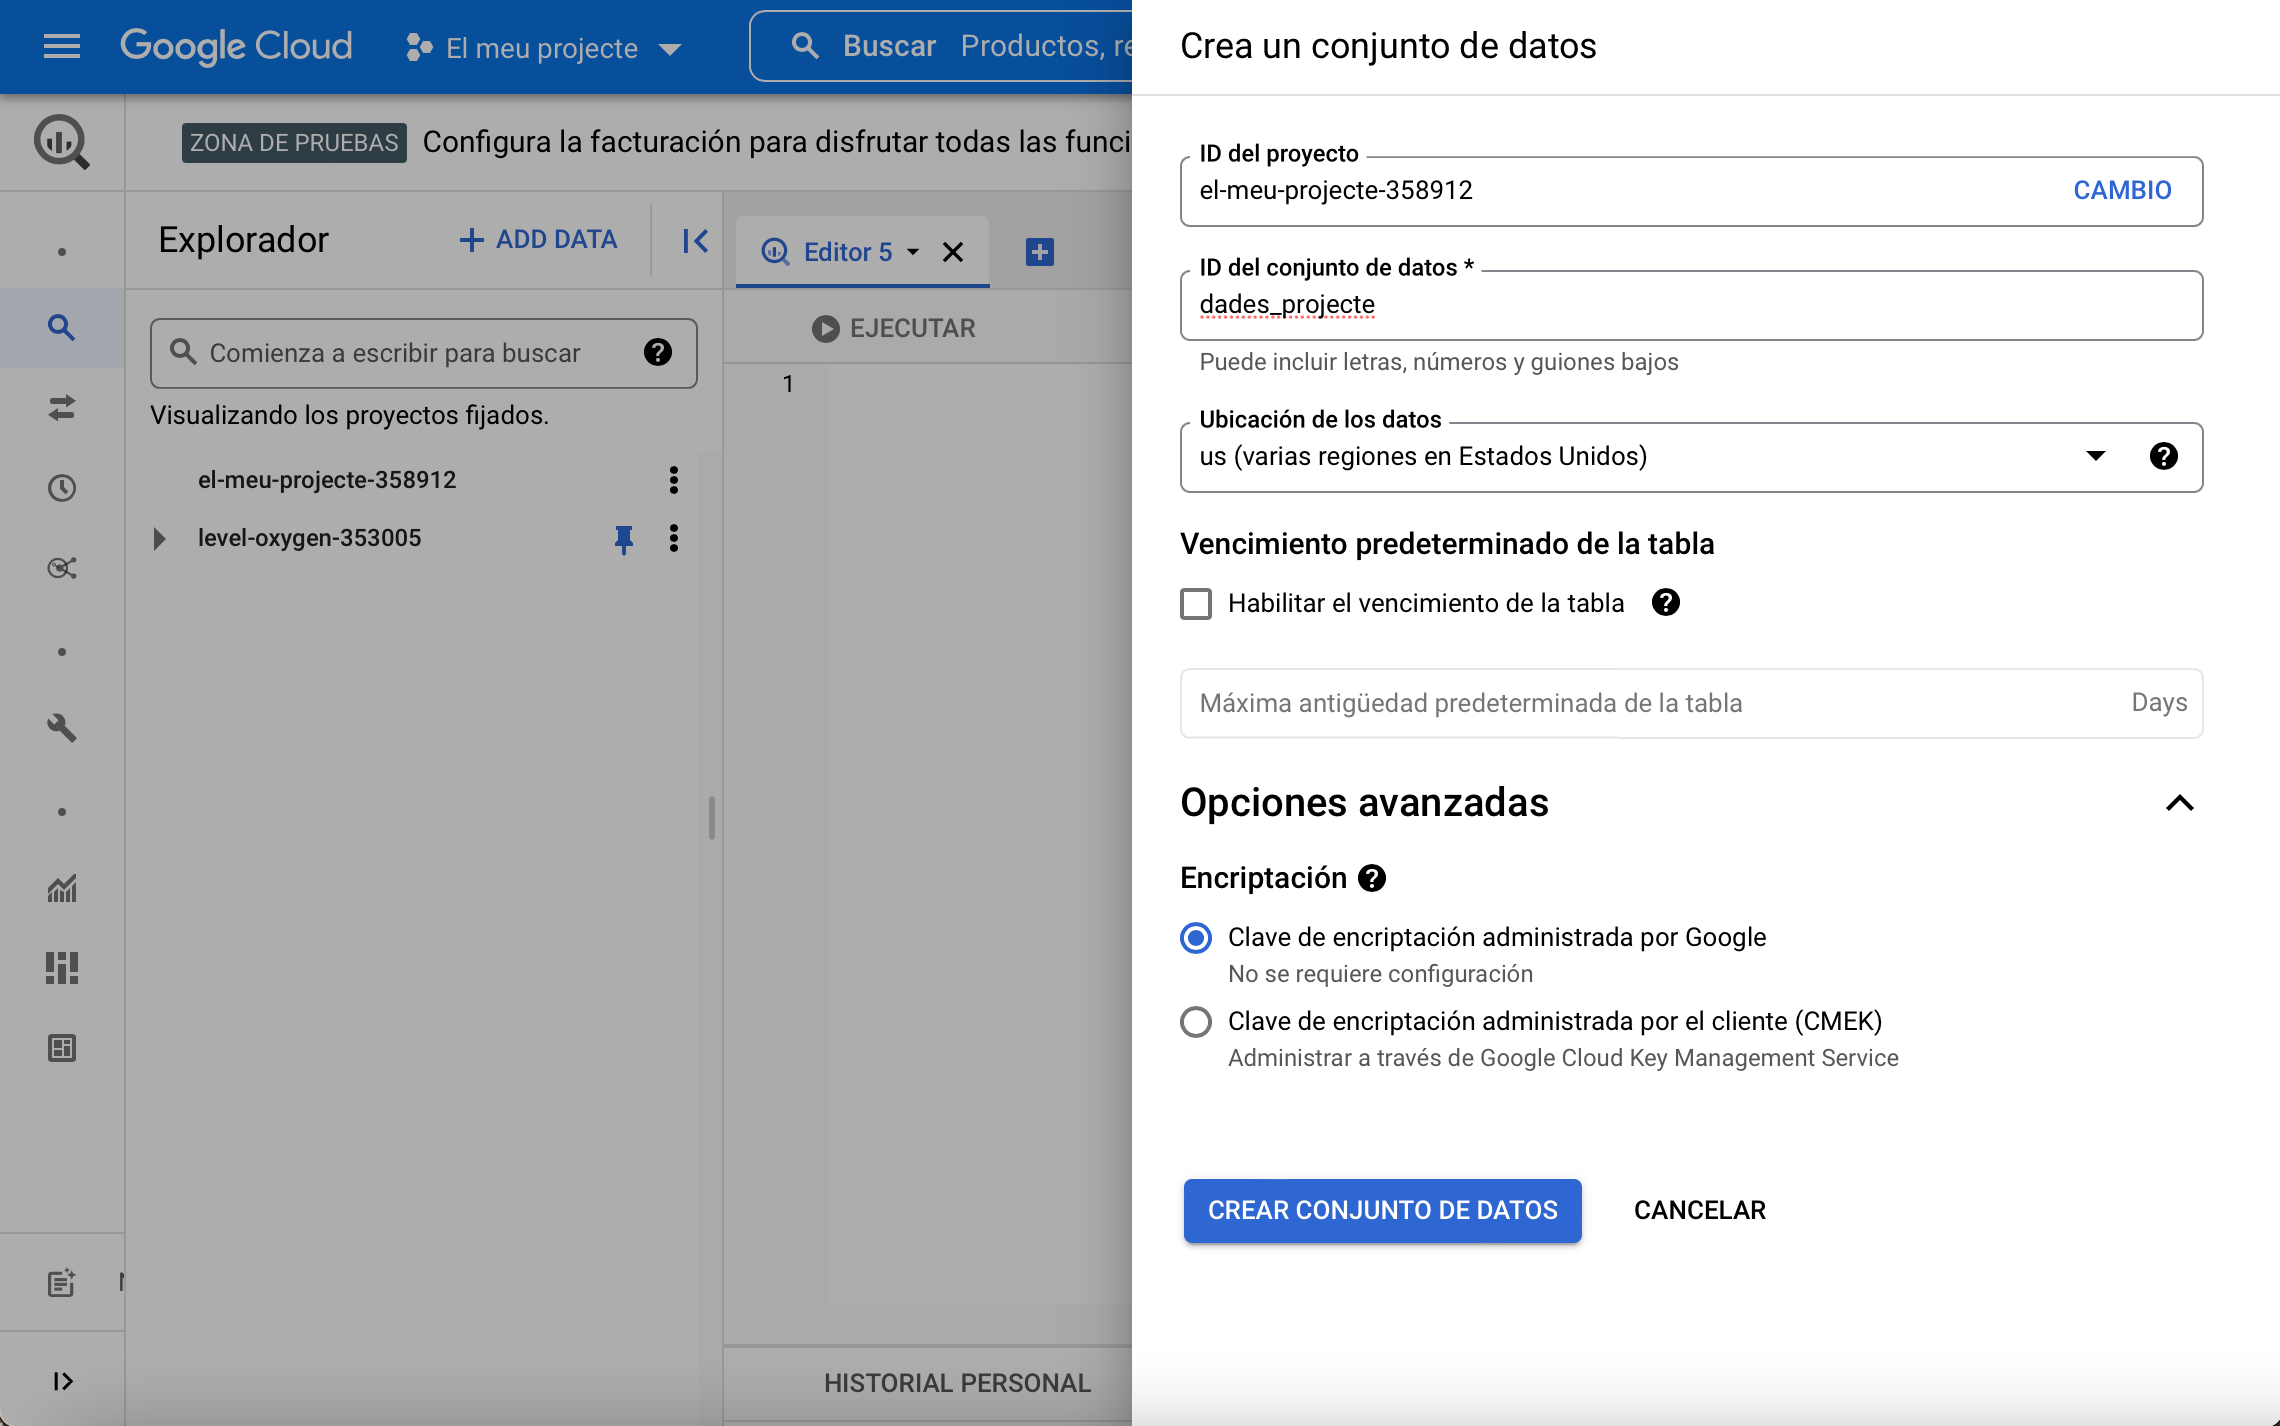
\includegraphics[width=7.25cm]{bq4}}%
\par
\caption{Creació d'un conjunt de dades}
\label{fig:bq3}
\end{figure}
\vspace{2mm}

Tal com es pot veure a la figura ~\ref{fig:bq3}, hem creat un nou conjunt de dades anomenat \verb|dades_projecte| que estarà ubicat en el projecte \verb|el_meu_projecte|, la ubicació de les dades la hem posat a diverses regions dels Estats Units i, per últim, no hem habilitat un temps de venciment de la taula, sinó que per defecte BigQuery l'emmagatzemarà per 60 dies.

\vspace{2mm}
\begin{figure}[h!]
\begin{center}
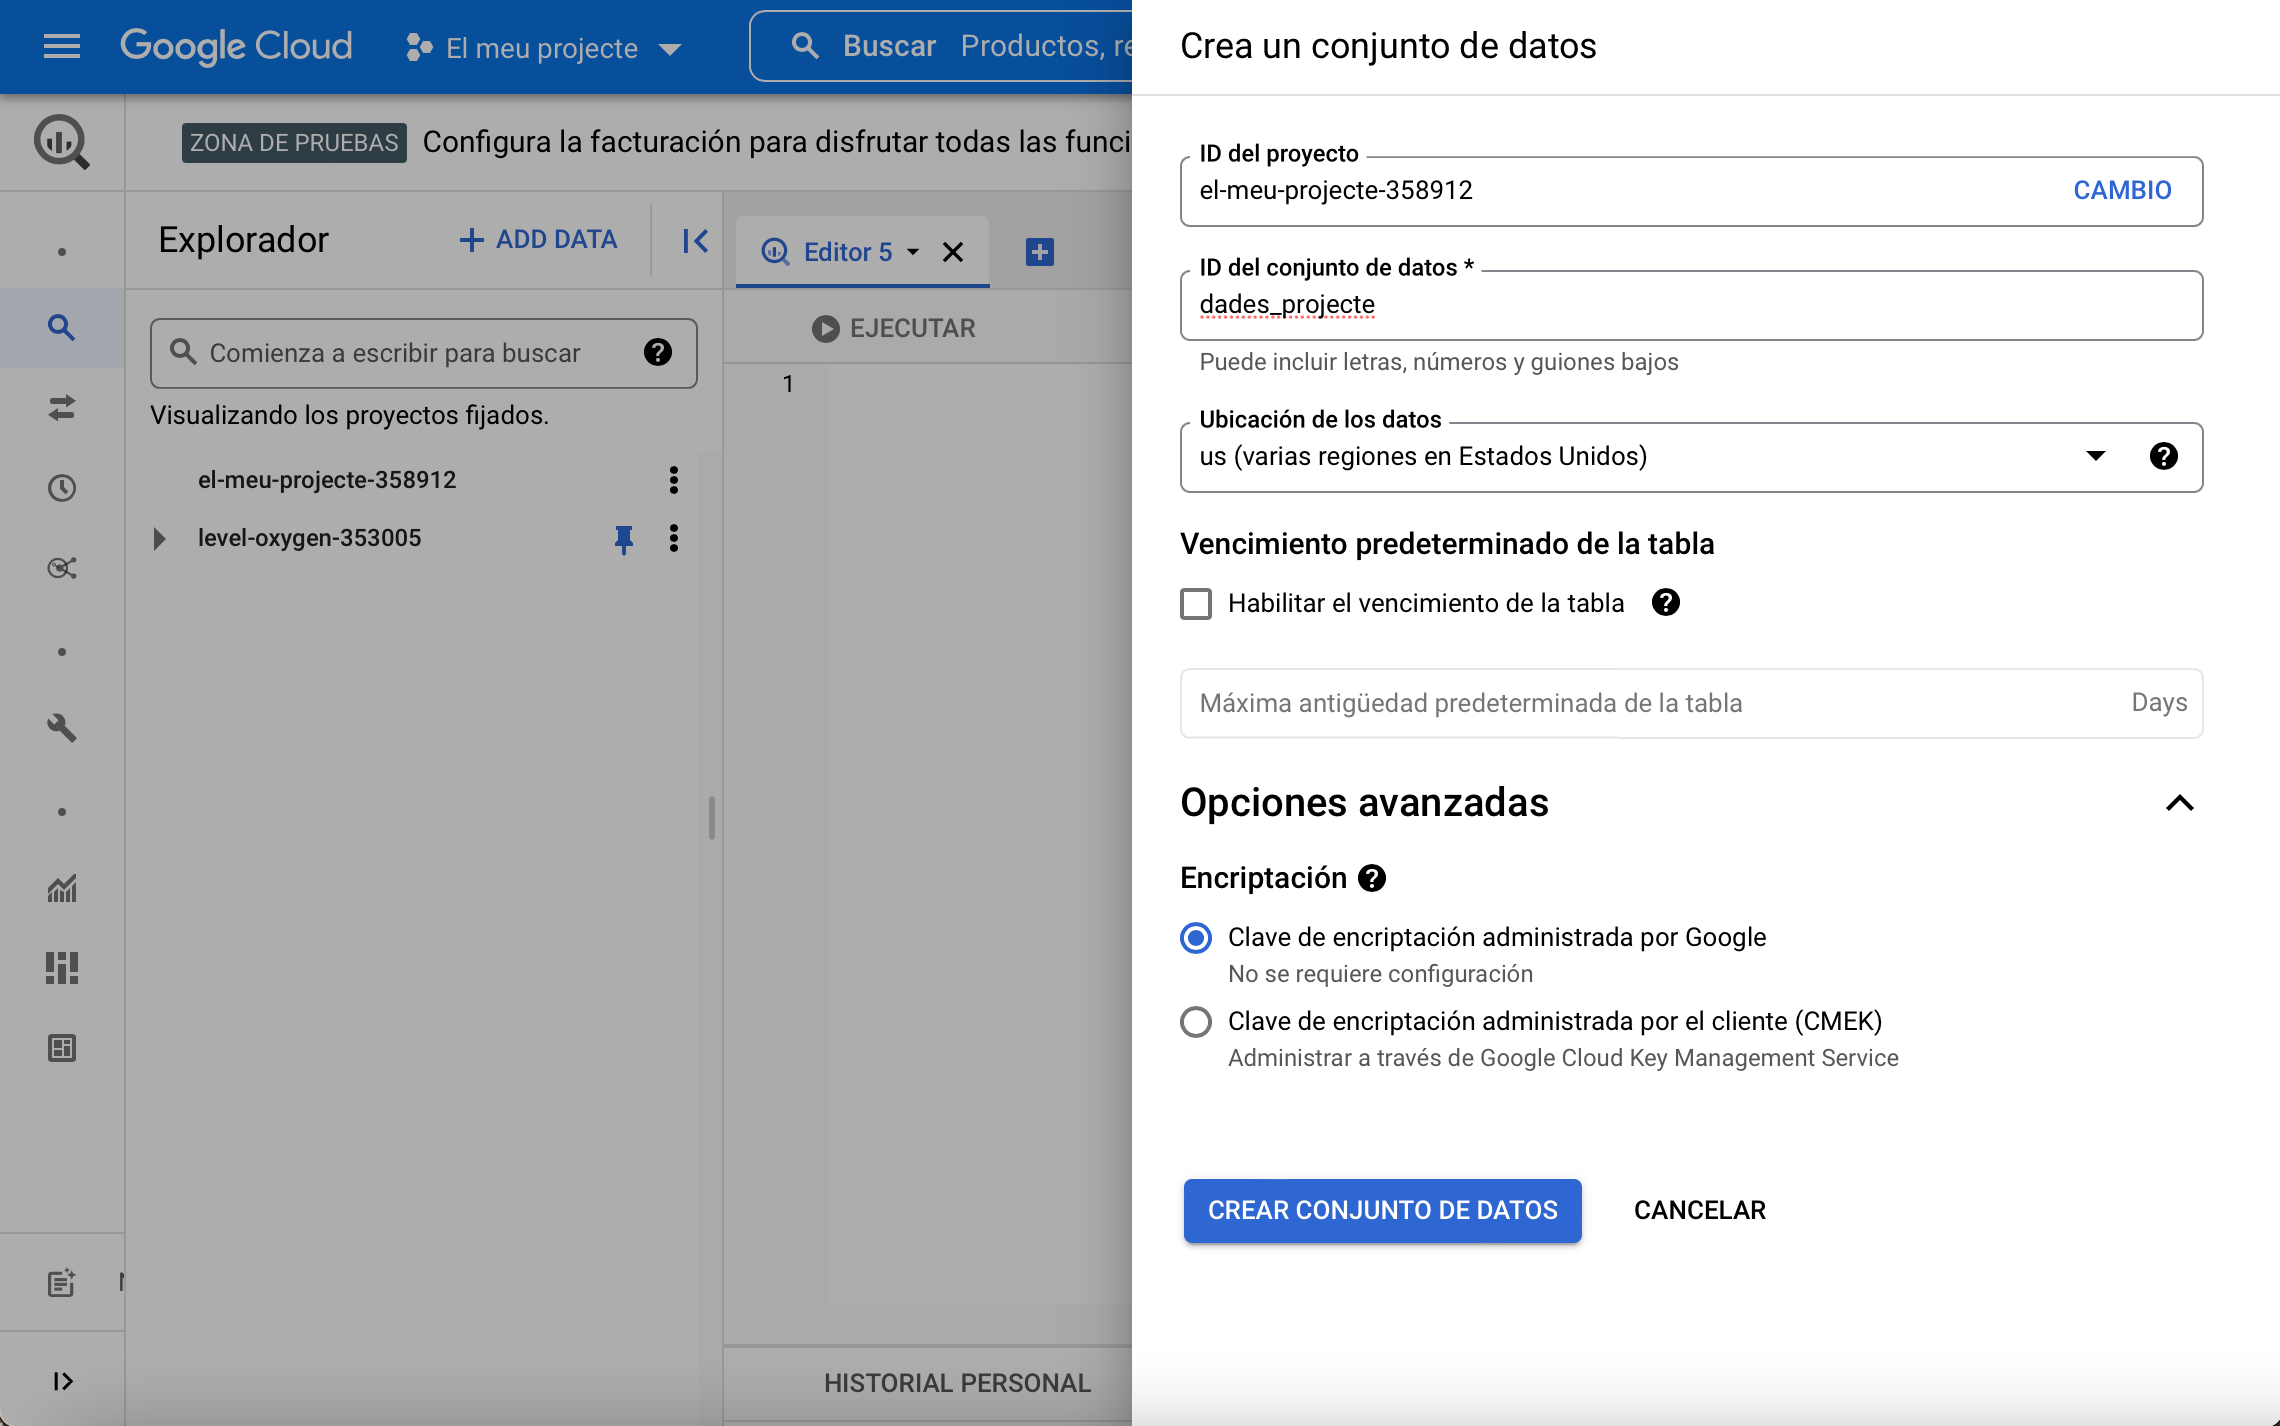
\includegraphics[width=10cm]{bq5}
\end{center}
\caption{Informació del conjunt de dades}
\label{fig:bq5}
\end{figure}
\vspace{2mm}

Un cop creat, el conjunt de dades \verb|dades_projecte|, es pot comprobar que ara apareix dins de \verb|el_meu_projecte| a la UI de BigQuery i, ampliant això, s'observa que no hi ha taules dins d'aquest. Ara, es pot donar un cop d'ull als detalls associats a aquest conjunt de dades (Figura ~\ref{fig:bq5}). Des d'aquest menú, podem triar obrir-lo, moment en el qual la informació del conjunt de dades apareix a la dreta. Aquí podem confirmar l'identificador del conjunt de dades, que també assenyala el projecte en el qual s'ha creat el conjunt de dades, i després altres detalls que inclouen les hores de creació i modificació, així com la ubicació d'aquest.

\vspace{2mm}

A més, des d'aquesta finestra podrem compartir el conjunt de dades amb altres usuaris. Hi ha opcions per a copiar i eliminar aquest conjunt de dades. I després, a la opció \textit{editar detalles}, podem reconfigurar el temps de caducitat de les taules, establir una descripció o afegir etiquetes. Per exemple, si volem marcar aquest conjunt de dades com a pertanyent a un equip, podem establir una etiqueta amb la clau d'equip i el valor corresponent. Després, quan guardem aquest conjunt de dades, les etiquetes apareixen a l'apartat de informació.

\subsection{Definició d'una taula de BigQuery des de la interfície d'usuari}

Després d'haver creat un conjunt de dades en un projecte, ja es pot crear una taula dins d'aquest conjunt de dades. Si tenim la informació del conjunt de dades, hauríem de veure aquesta opció per a crear una nova taula des d'aquí. Alternativament, podem dirigir-nos al projecte, després al conjunt de dades i triar l'opció de crear una taula. Apareixerà un formulari i tindrem l'opció d'especificar una font per a la nostra taula. Això ens permetrà extreure dades de fonts ja existents, com l'emmagatzematge en el núvol de Google o bé un arxiu dels nostres propis sistemes. La primera taula que crearem serà bastant simple, i ens servirà per explorar una mica la plataforma. De fet, serà una taula buida anomenada \verb|accidents| (Figura ~\ref{fig:bq6}). 

\vspace{2mm}
\begin{figure}[h!]
\par
\raisebox{-.5\height}{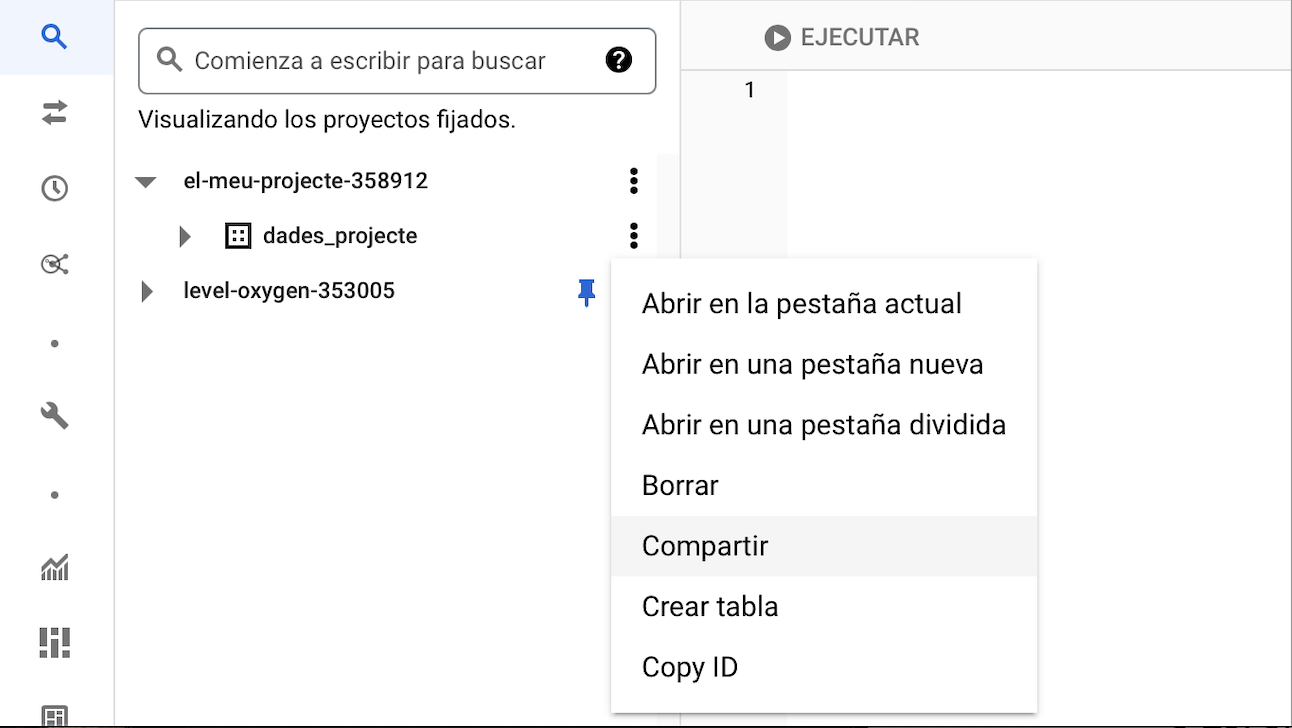
\includegraphics[width=7.25cm]{bq6}}%
\hfill
\raisebox{-.5\height}{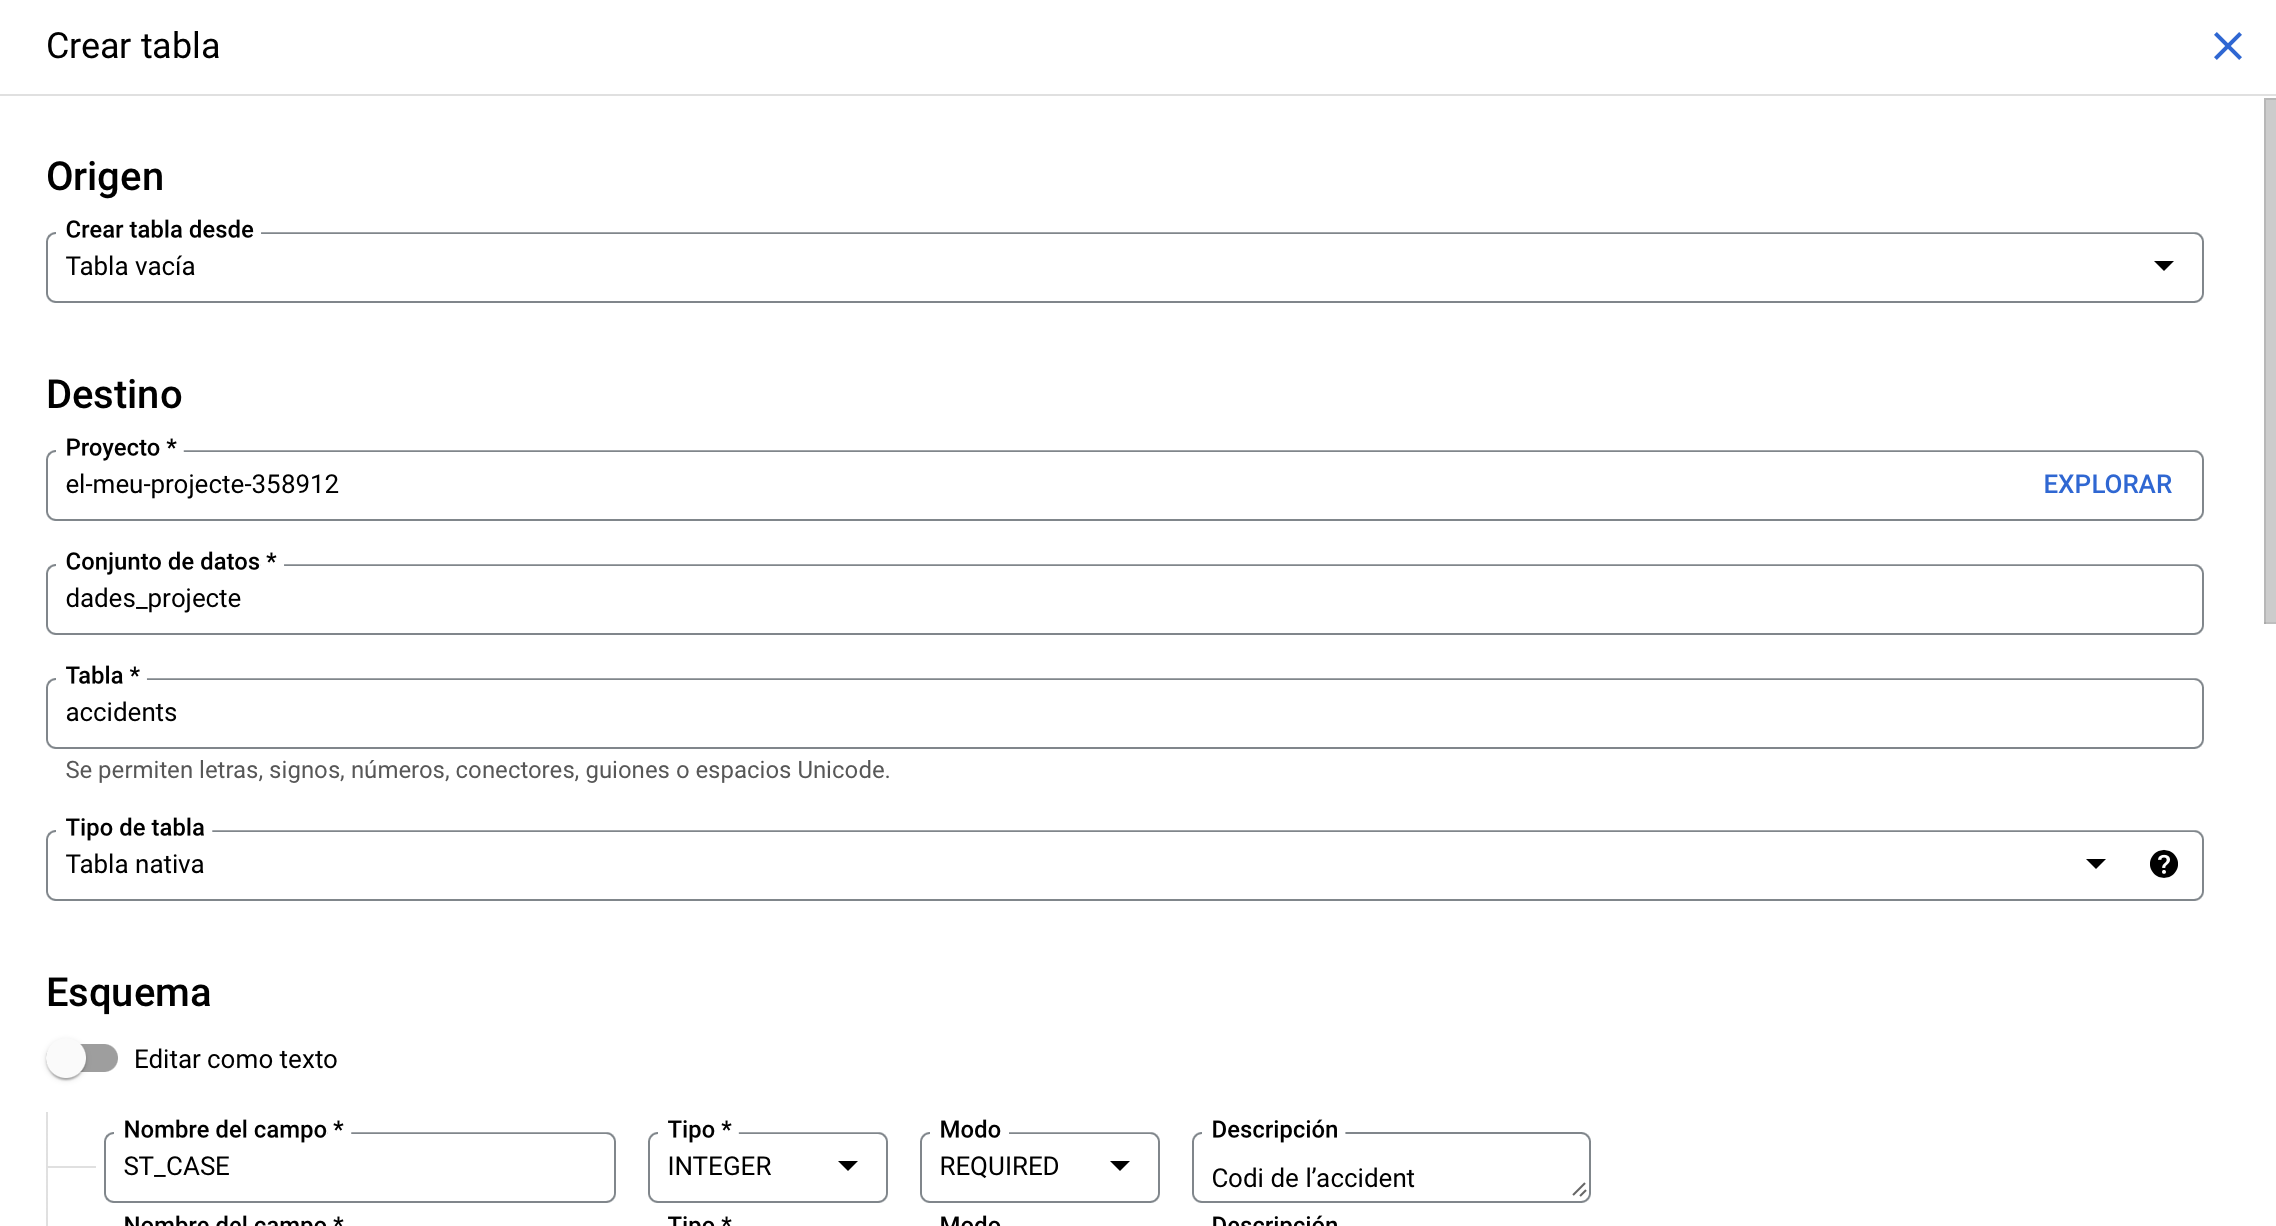
\includegraphics[width=7.25cm]{bq7 copia}}%
\par
\caption{Creació d'una taula}
\label{fig:bq6}
\end{figure}
\vspace{2mm}

A continuació, passem a la secció d'Esquema. Podem fer ús d'aquesta interfície per a establir les columnes de la nostra taula, incloent-hi els tipus i altres configuracions. La primera columna que definiré és l'identificador de l'accident, que s'anomenarà \verb|ST_CASE|. Per al tipus de variable, podem triar d'entre menú d'opcions, que inclou tots els tipus amb els quals ja estem familiaritzats. Quant a la manera (columna \textit{modo} a la figura ~\ref{fig:bq8}), aquesta determinarà si els valors d'aquesta columna poden ser nuls o si es requereix un valor (com és el cas de l'identificador), així com també podem establir que els valors siguin d'un tipus que es pugui repetir, marcant \textit{indistint}. Finalment, es pot escriure una descripció per a la variable, que és opcional. 

\vspace{2mm}
\begin{figure}[h!]
\begin{center}
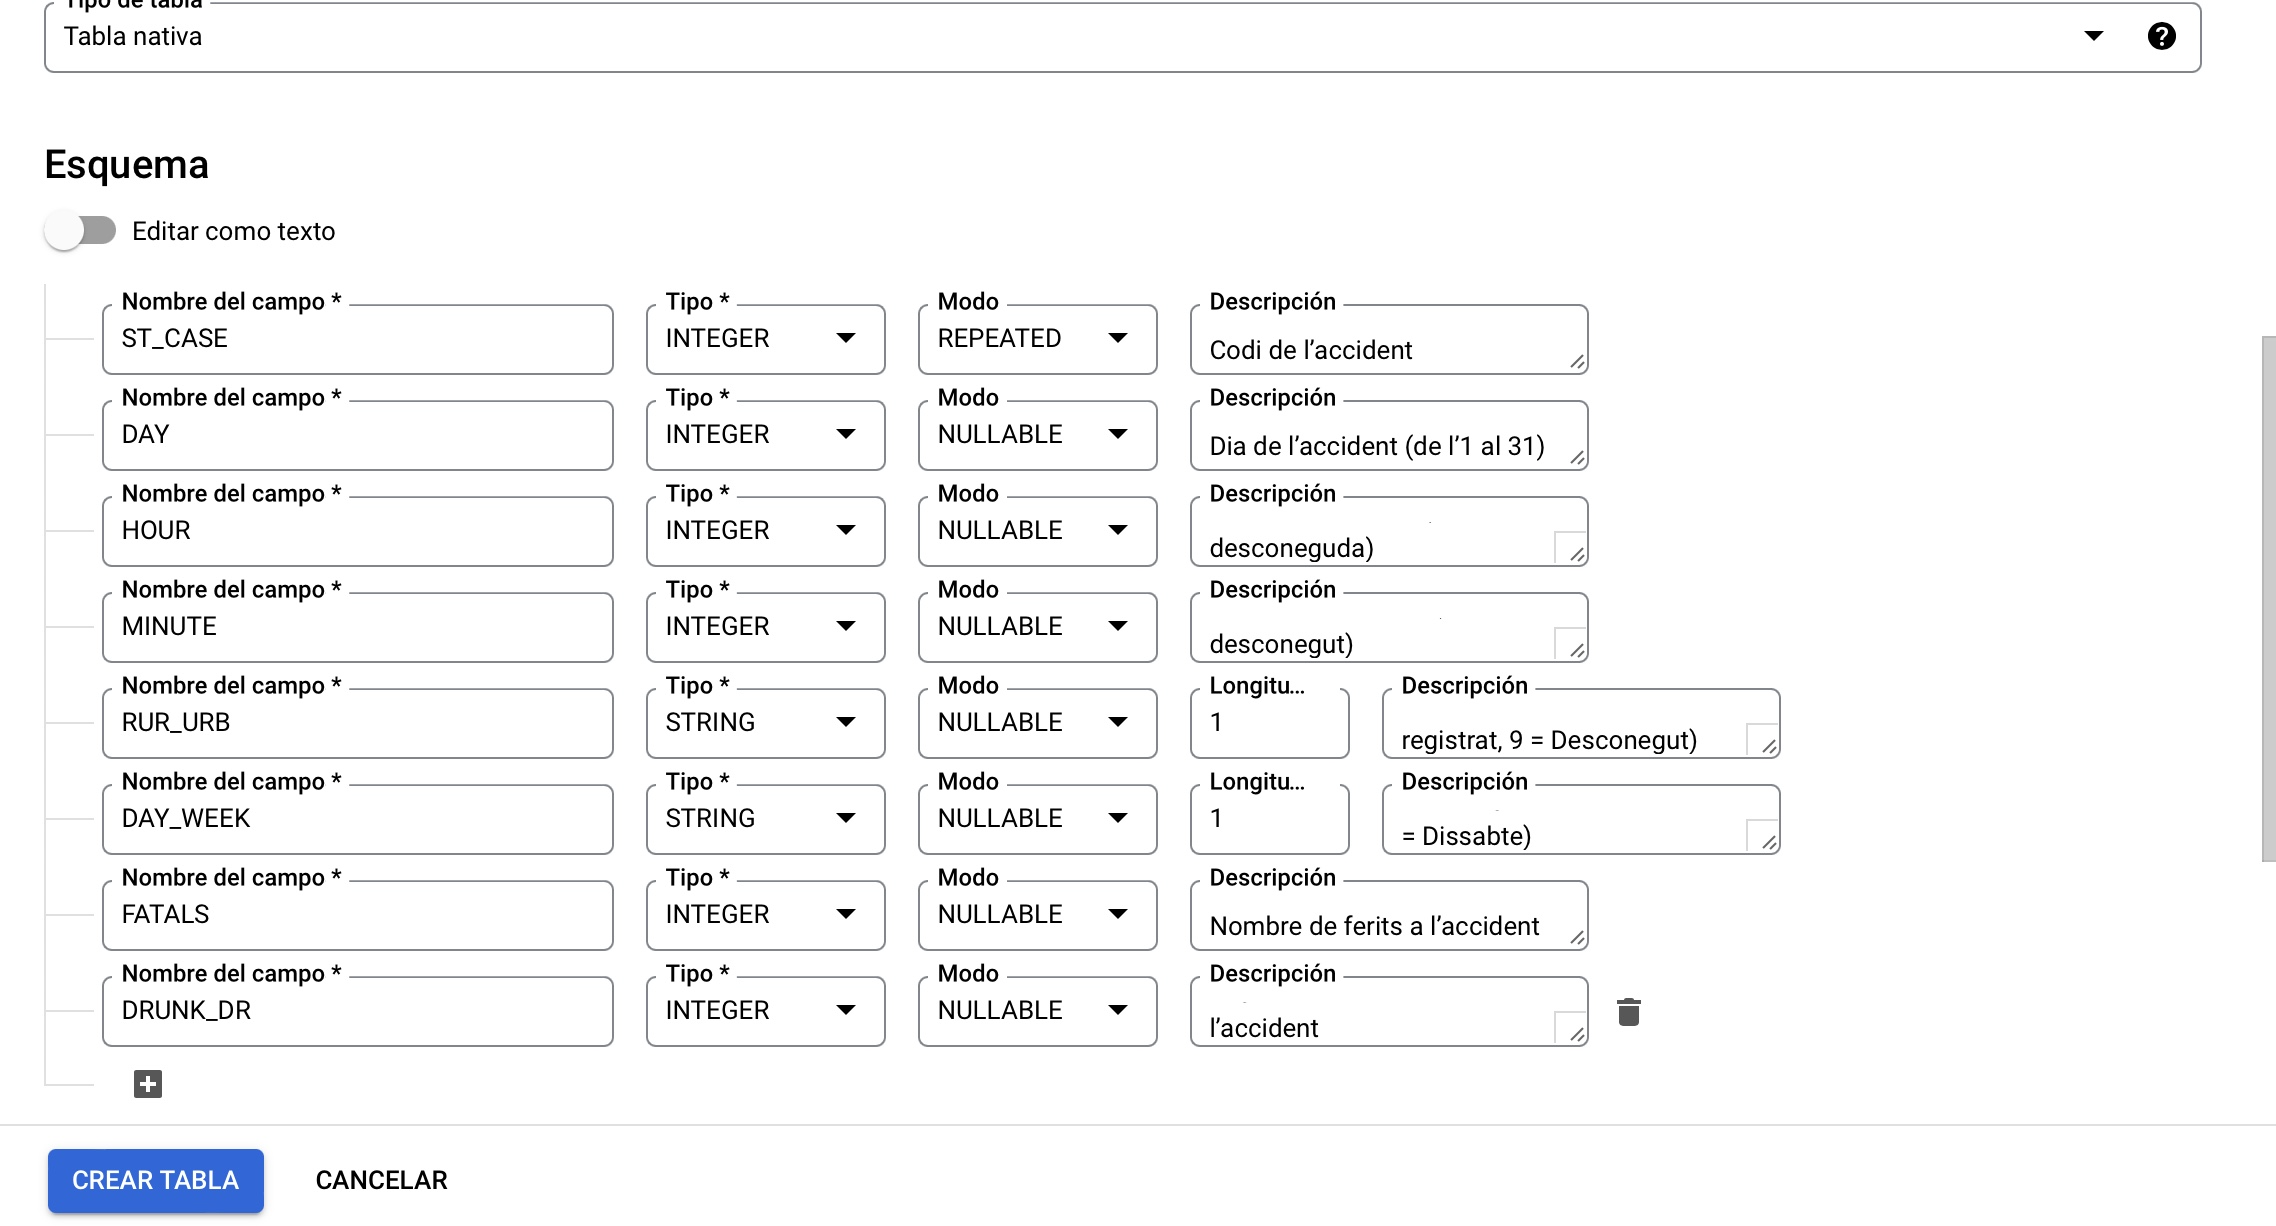
\includegraphics[width=10cm]{bq8}
\end{center}
\caption{Esquema de la nostra taula}
\label{fig:bq8}
\end{figure}
\vspace{2mm}

La taula ~\ref{tab:taula1} que acabem de crear està formada per 8 variables, 6 de les quals són numèriques i 2 categòriques, i es descriuen tal i com es pot veure a continuació.

\begin{table}[h]
\resizebox{\textwidth}{!}{%
\begin{tabular}{|l|l|l|}
\hline
Variable  & Tipus      & Descripció                                                                                                        \\ \hline
ST\_CASE       & Numèrica & Codi de l'accident                                                                                   \\ \hline
DAY       & Numèrica & Dia de l’accident (de l’1 al 31)                                                                                    \\ \hline
HOUR      & Numèrica   & Hora de l’accident (99 = desconeguda)                                                                               \\ \hline
MINUTE    & Numèrica   & Minut de l’accident (99 = desconegut)                                                                               \\ \hline
RUR\_URB  & Categòrica & Informació sobre la localització (1 = Rural, 2 = Urbà, 6 = Via no classificada, 8 = No registrat, 9 = Desconegut)   \\ \hline
DAY\_WEEK & Categòrica & Dia de la setmana (1 = Diumenge, 2 = Dilluns, ..., 7 = Dissabte)                                                    \\ \hline
FATALS    & Numèrica   & Nombre de ferits a l’accident                                                                                       \\ \hline
DRUNK\_DR & Numèrica   & Nombre de conductors beguts involucrats a l’accident                                                                \\ \hline
\end{tabular}%
}
\caption{Especificacions de la taula Accidents}
\label{tab:taula1}
\end{table}

\vspace{2mm}

En el transcurs del treball, farem ús d'aquesta taula, juntament amb dues més, que prenen de nom de \verb|persones| i \verb|vehicles|, per analitzar les dades que es van prendre d'un conjunt d'accidents que es van donar als Estats Units. 

\subsubsection{Afegir dades a una taula de BigQuery senzilla}

Ara que hem creat una taula de consulta, podem centrar-nos en treballar amb ella. Per a això, ens desplaçarem cap avall i donarem un cop d'ull al primer esquema de la taula (a la figura ~\ref{fig:bq9}), on es troba a alguna informació interessant. Més enllà de la identificació de la taula, a l'esquerra de la figura, també podem comprovar la grandària de la taula a la dreta, que ens donarà una indicació de la quantitat de dades que es processaran, si anéssim a executar consultes sobre aquesta. La grandària d'emmagatzematge a llarg termini assenyala les dades a les quals no s'ha accedit en els últims 90 dies, i després, per descomptat, tenim les hores de creació i modificació juntament amb la ubicació de les dades de la taula. Des d'aquesta interfície, també podem editar els detalls existents d'aquesta taula. Aquí podem establir un temps de caducitat en cas que vulguem anul·lar el que s'ha establert en el nivell del conjunt de dades. També tenim l'opció d'establir una descripció o afegir etiquetes.

\vspace{2mm}
\begin{figure}[h!]
\par
\raisebox{-.5\height}{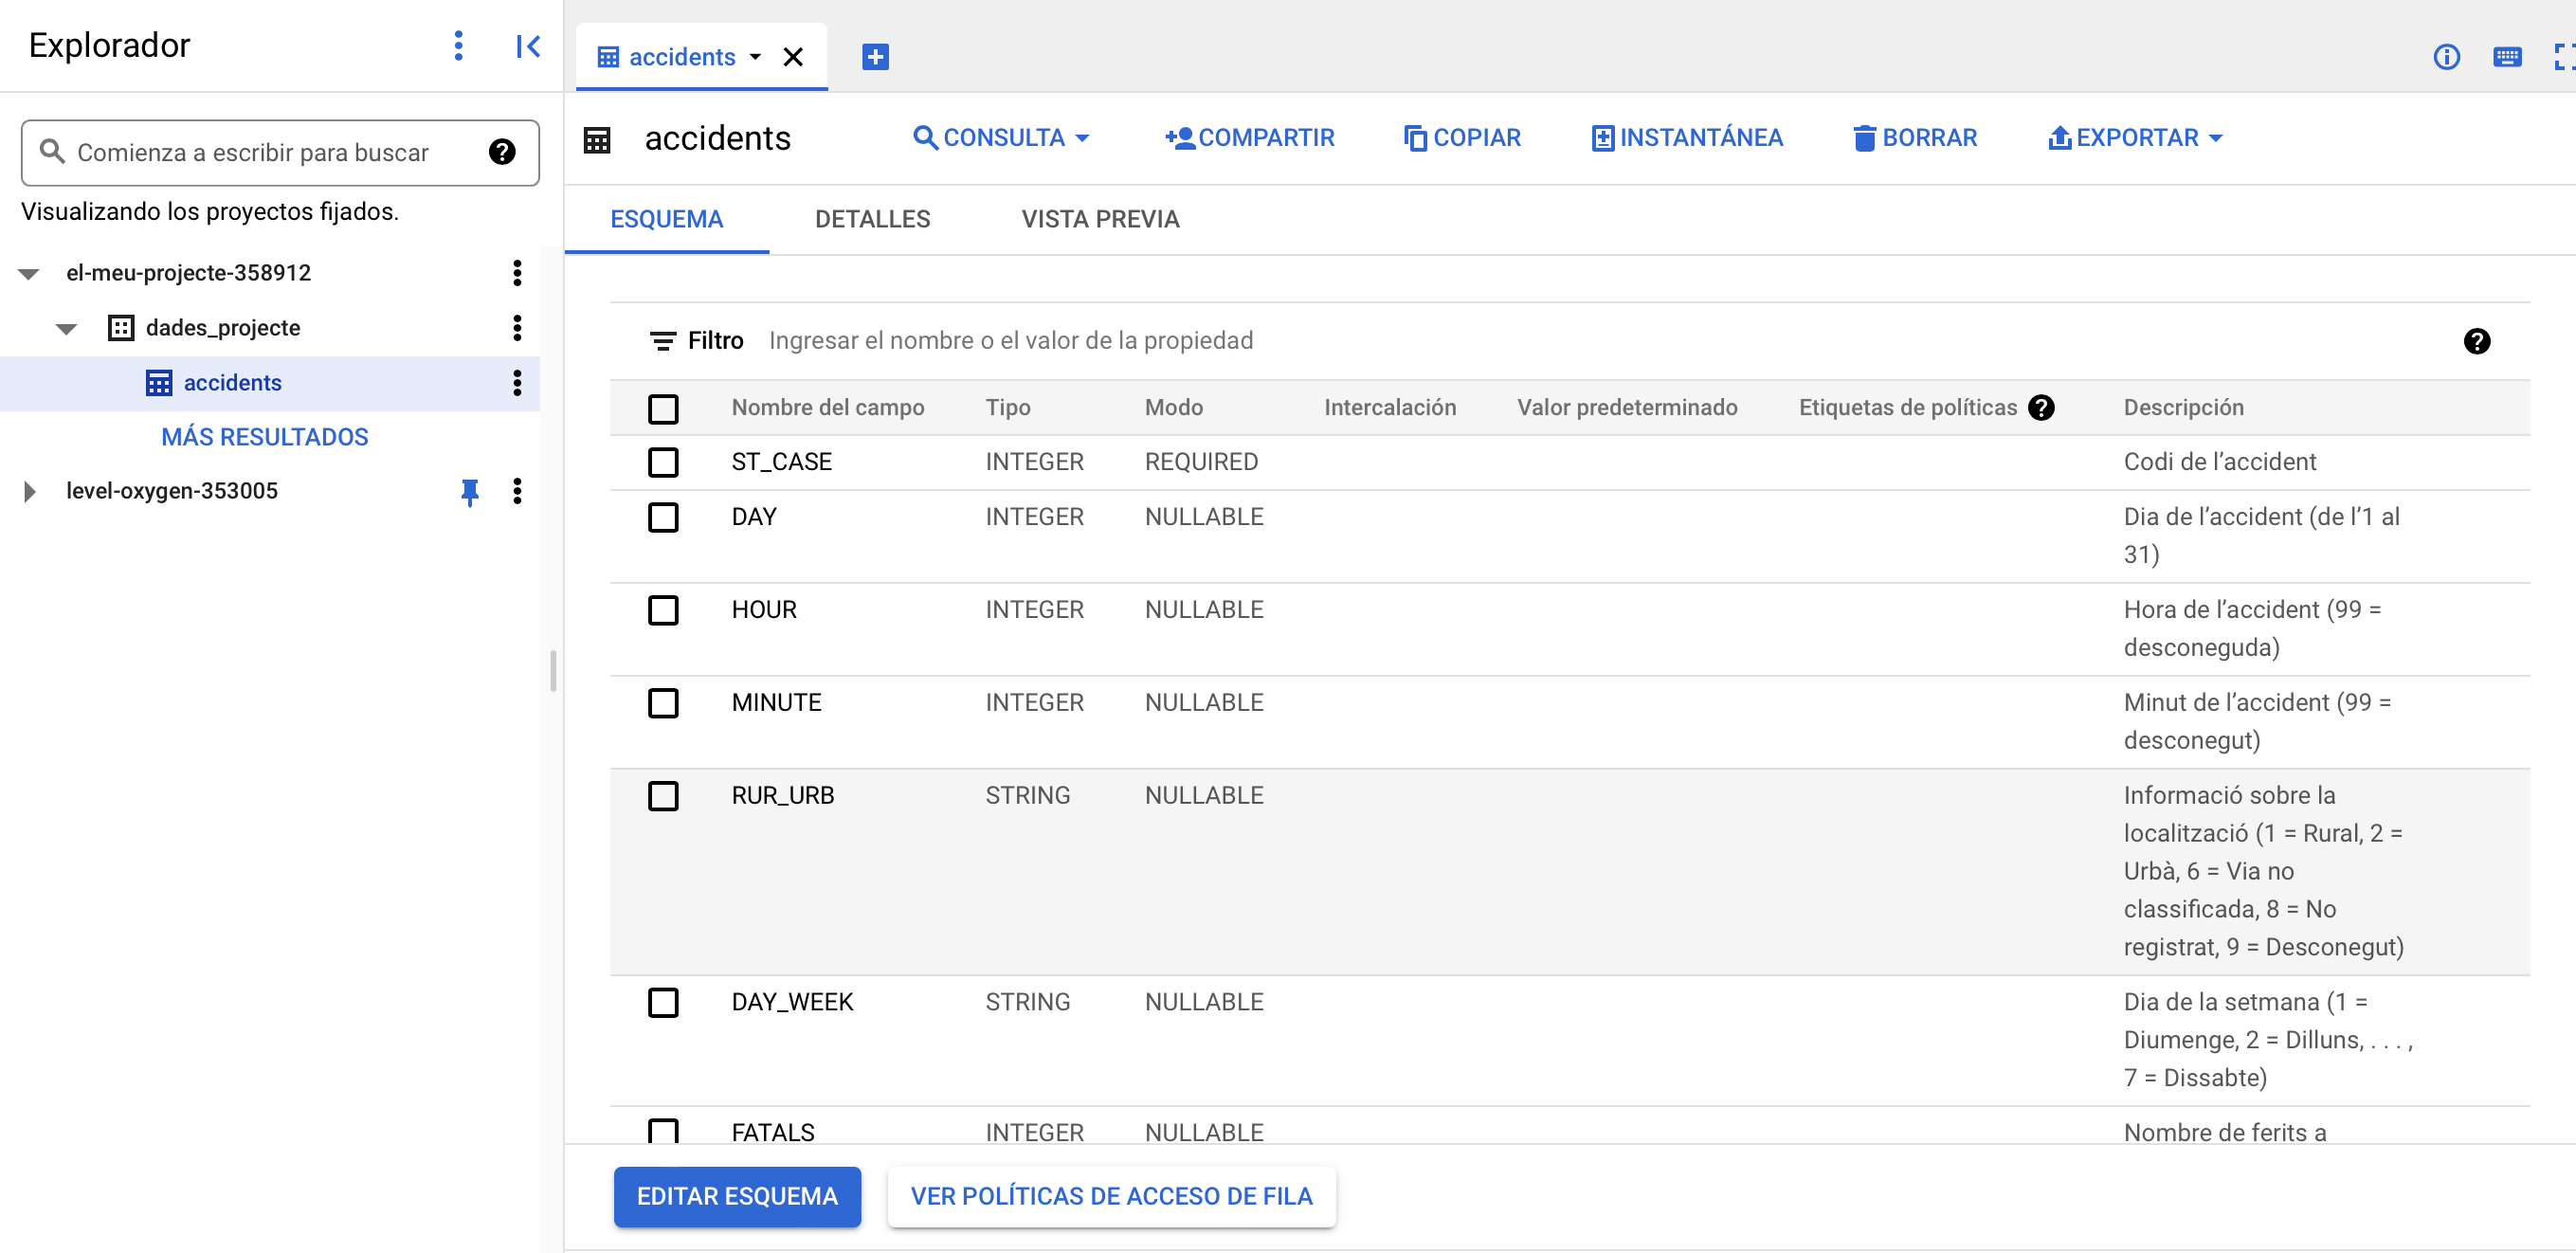
\includegraphics[width=7.25cm]{bq9}}%
\hfill
\raisebox{-.5\height}{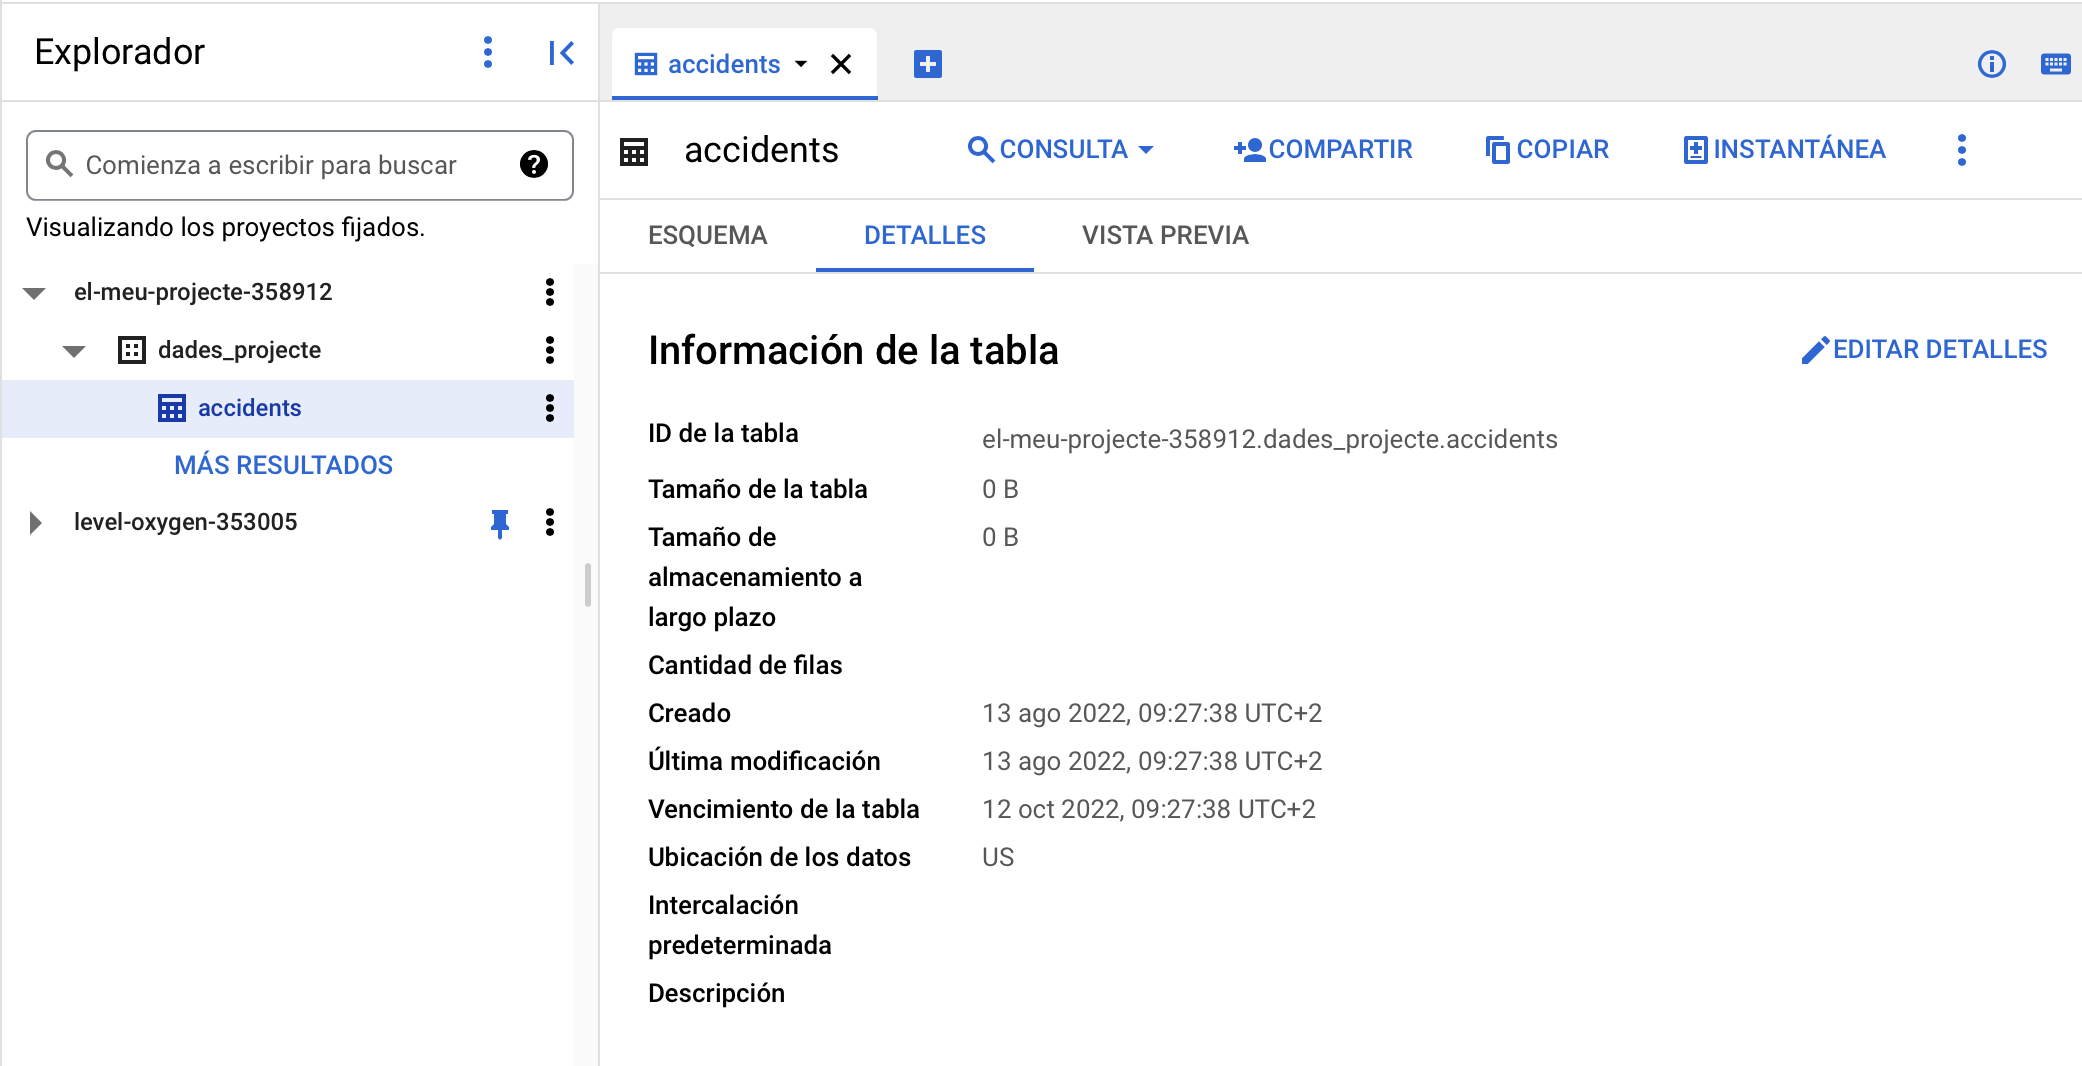
\includegraphics[width=7.25cm]{bq10}}%
\par

\caption{Detalls de la taula}
\label{fig:bq9}
\end{figure}
\vspace{2mm}

Una altra característica que podem consultar és la vista prèvia de la taula, i com és lògic, veurem que aquesta encara no conté dades, ja que simplement hem creat l'esquema de la taula, sense inserir cap dada en aquesta. Si féssim ús de SQL, en qualsevol altre context es pdrien afegir dades a partir d'una simple consulta a la taula, que tindria l'estructura següent:

\begin{verbatim}
INSERT INTO `el-meu-projecte-358912.dades_projecte.accidents` 
(ST_CASE, DAY, HOUR, MINUTE, RUR_URB, DAY_WEEK, FATALS, DRUNK_DR)
VALUES (20055, 1, 20, 55, "1", "3", 3, 0);
\end{verbatim}

A partir d'aquesta consulta afegiriem a la taula el cas d'un accident amb identificador 20055, que es va produir el dia 1 del mes a les 20:55 a una zona rural (\verb|RUR_URB| = 1)un dimarts (\verb|DAY_WEEK| = 3), i en el que hi ha 3 ferits i cap conductor begut involucrat en l'accident.

Això no obstant, quan intentem executar la consulta, BigQuery ens informa d'un error (Figura ~\ref{fig:bq11}). Si recordem, prèviament s'han definit algunes de les limitacions per a l'ús de la zona de proves de BigQuery. Entre aquestes s´hi troba que no podem utilitzar el llenguatge de manipulació de dades (DML), és a dir, que no podem modificar la taula amb sentències com \verb|INSERT INTO|, \verb|UPDATE| o \verb|DELETE|, per exemple.Per aquest motiu, l'error ens avisa de que no tenim el nostre projecte vinculat a un compte i, per tant, no ens avaluarà la nostra consulta.

\vspace{2mm}
\begin{figure}[h!]
\begin{center}
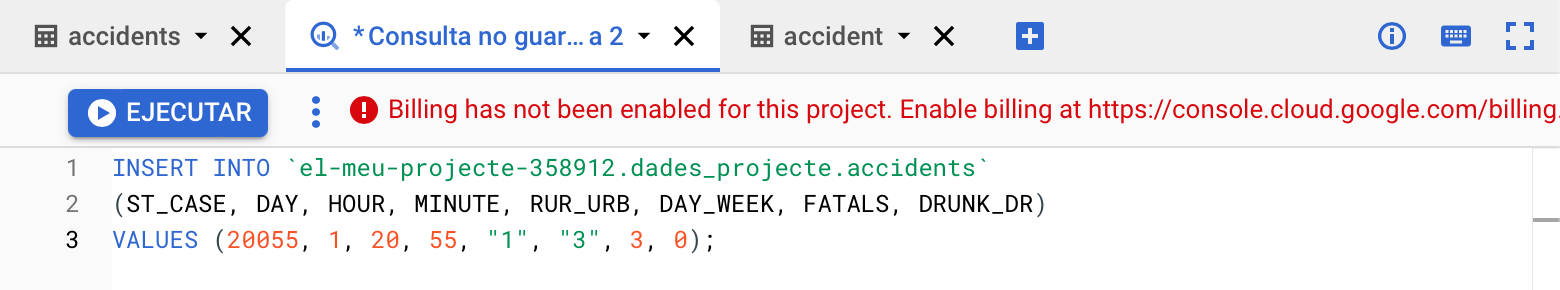
\includegraphics[width=12cm]{bq11}
\end{center}
\caption{Inserció de dades a la taula}
\label{fig:bq11}
\end{figure}
\vspace{2mm}

\subsection{Càrrega de dades per crear una taula de BigQuery}

Hem vist que és possible crear una taula buida, però que la zona de proves (\textit{sandbox}) no ens permet després emplenar-la amb dades amb sentències \verb|INSERT|. Ara explorarem un cas d'ús més comú per als usuaris de BigQuery en el qual es crea una taula a partir de dades existents. Per a això, ens dirigirem al nostre conjunt de dades, \verb|dades_projecte|, i triarem crear una nova taula. Aquesta cop, la font no serà una taula buida, sinó que carregarem un arxiu CSV del nostre propi sistema d'arxius. Un cop seleccionem importar les dades, es pot seleccionar diferents tipus d'arxiu com ara CSV, JSON, Avro o Parquet, principalment. Per a respectar les limitacions de la zona de proves, hi ha algunes restriccions quant a la grandària de l'arxiu que podem pujar, recordem que aquestes han de ser menors a 10 Gb. Procedim llavors a navegar pels nostres sistemes d'arxius per a l'arxiu a pujar. Una vegada que l'arxiu ha estat seleccionat, el format de l'arxiu s'ha establert automàticament en CSV (Figura ~\ref{fig:bq12}). 

\vspace{2mm}
\begin{figure}[h!]
\par
\raisebox{-.5\height}{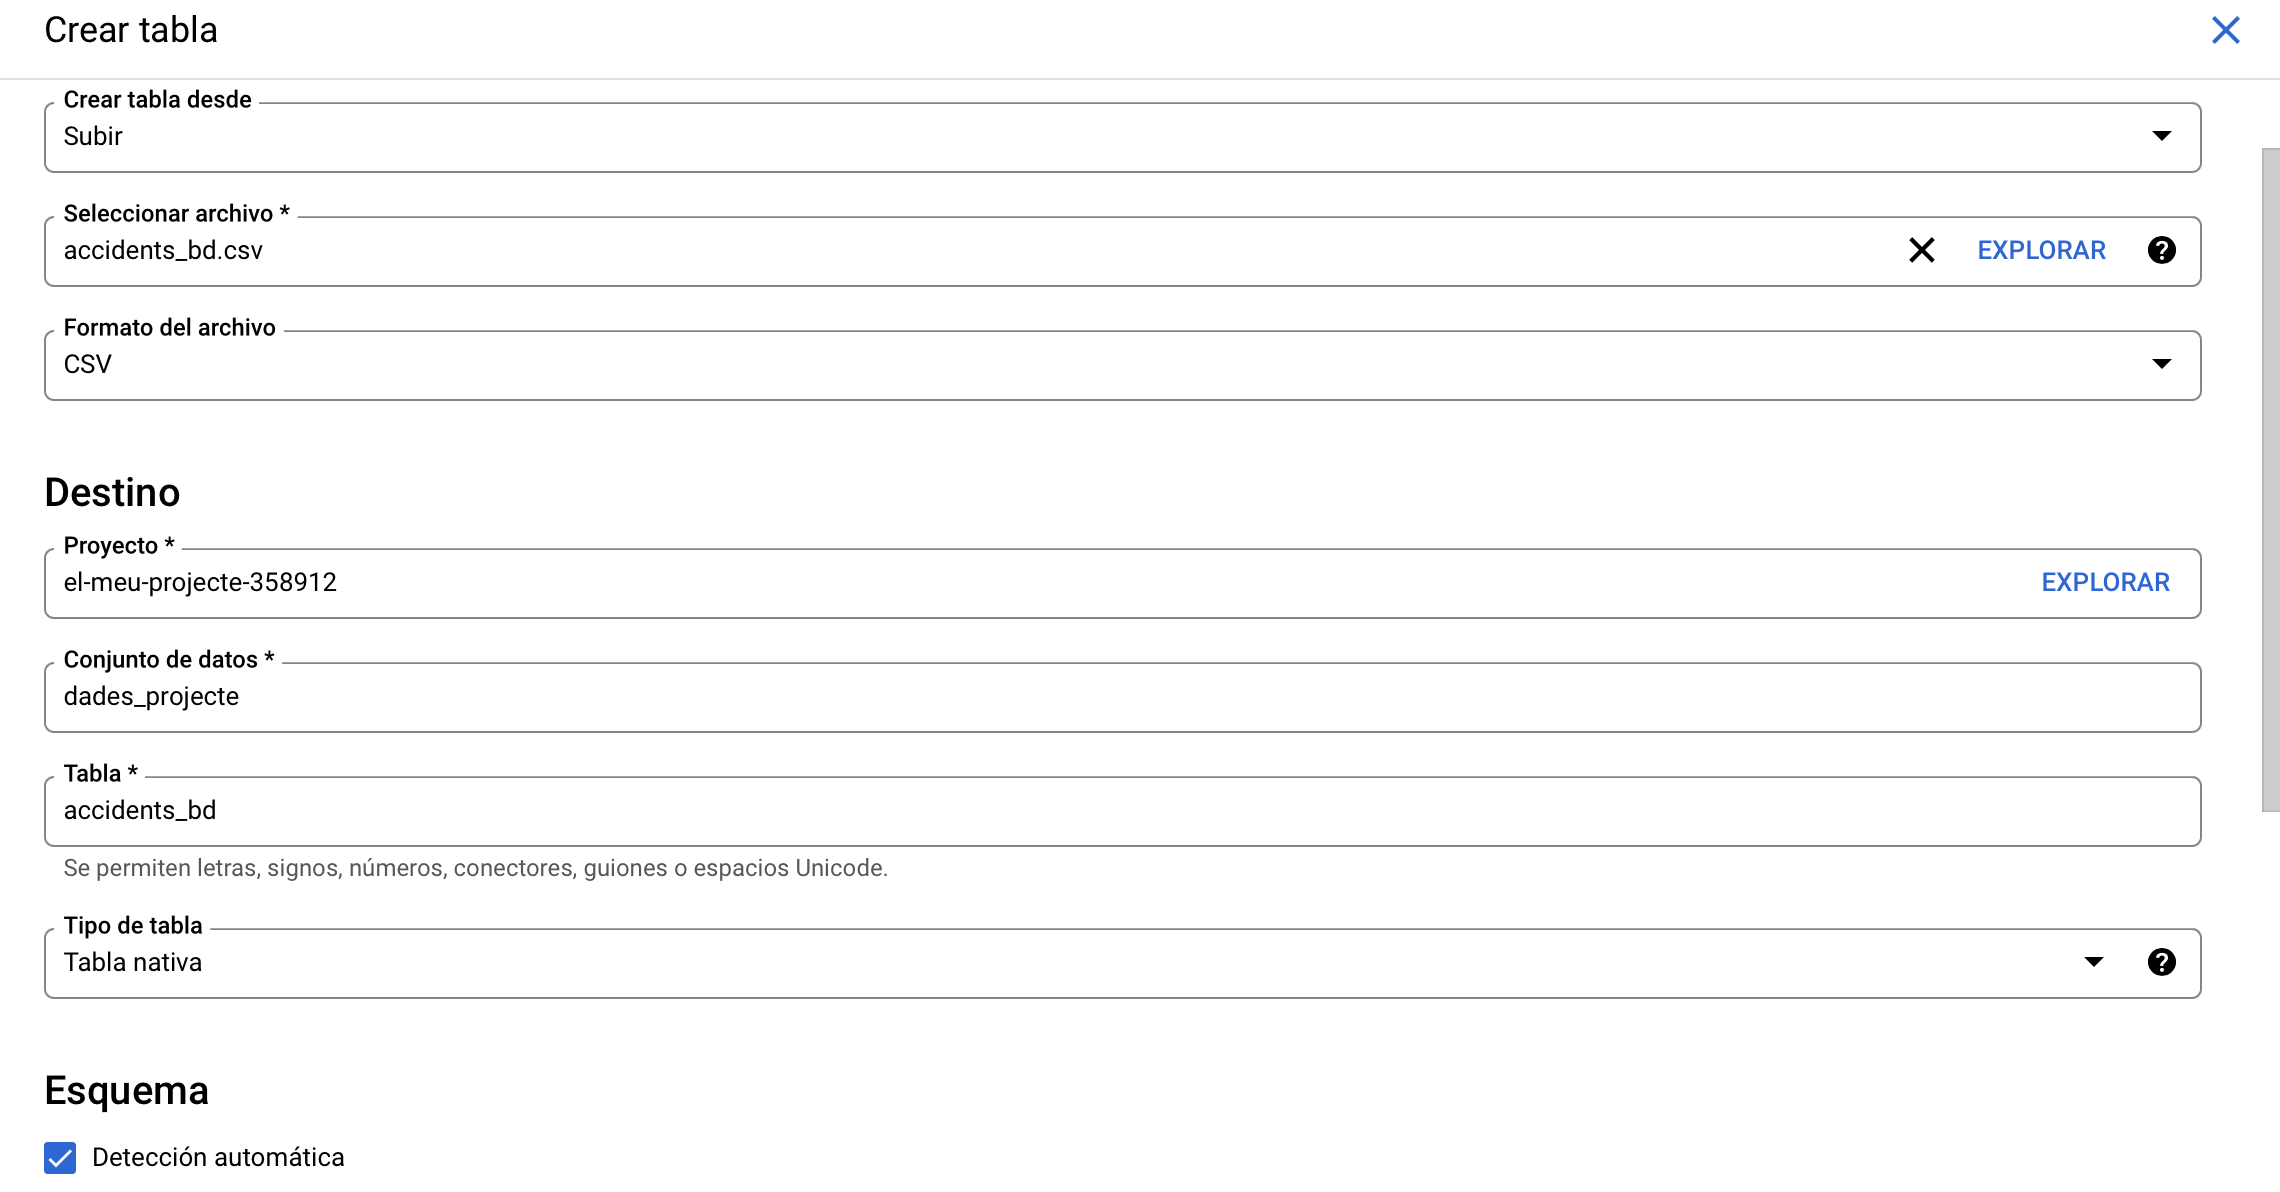
\includegraphics[width=7.25cm]{bq12}}%
\hfill
\raisebox{-.5\height}{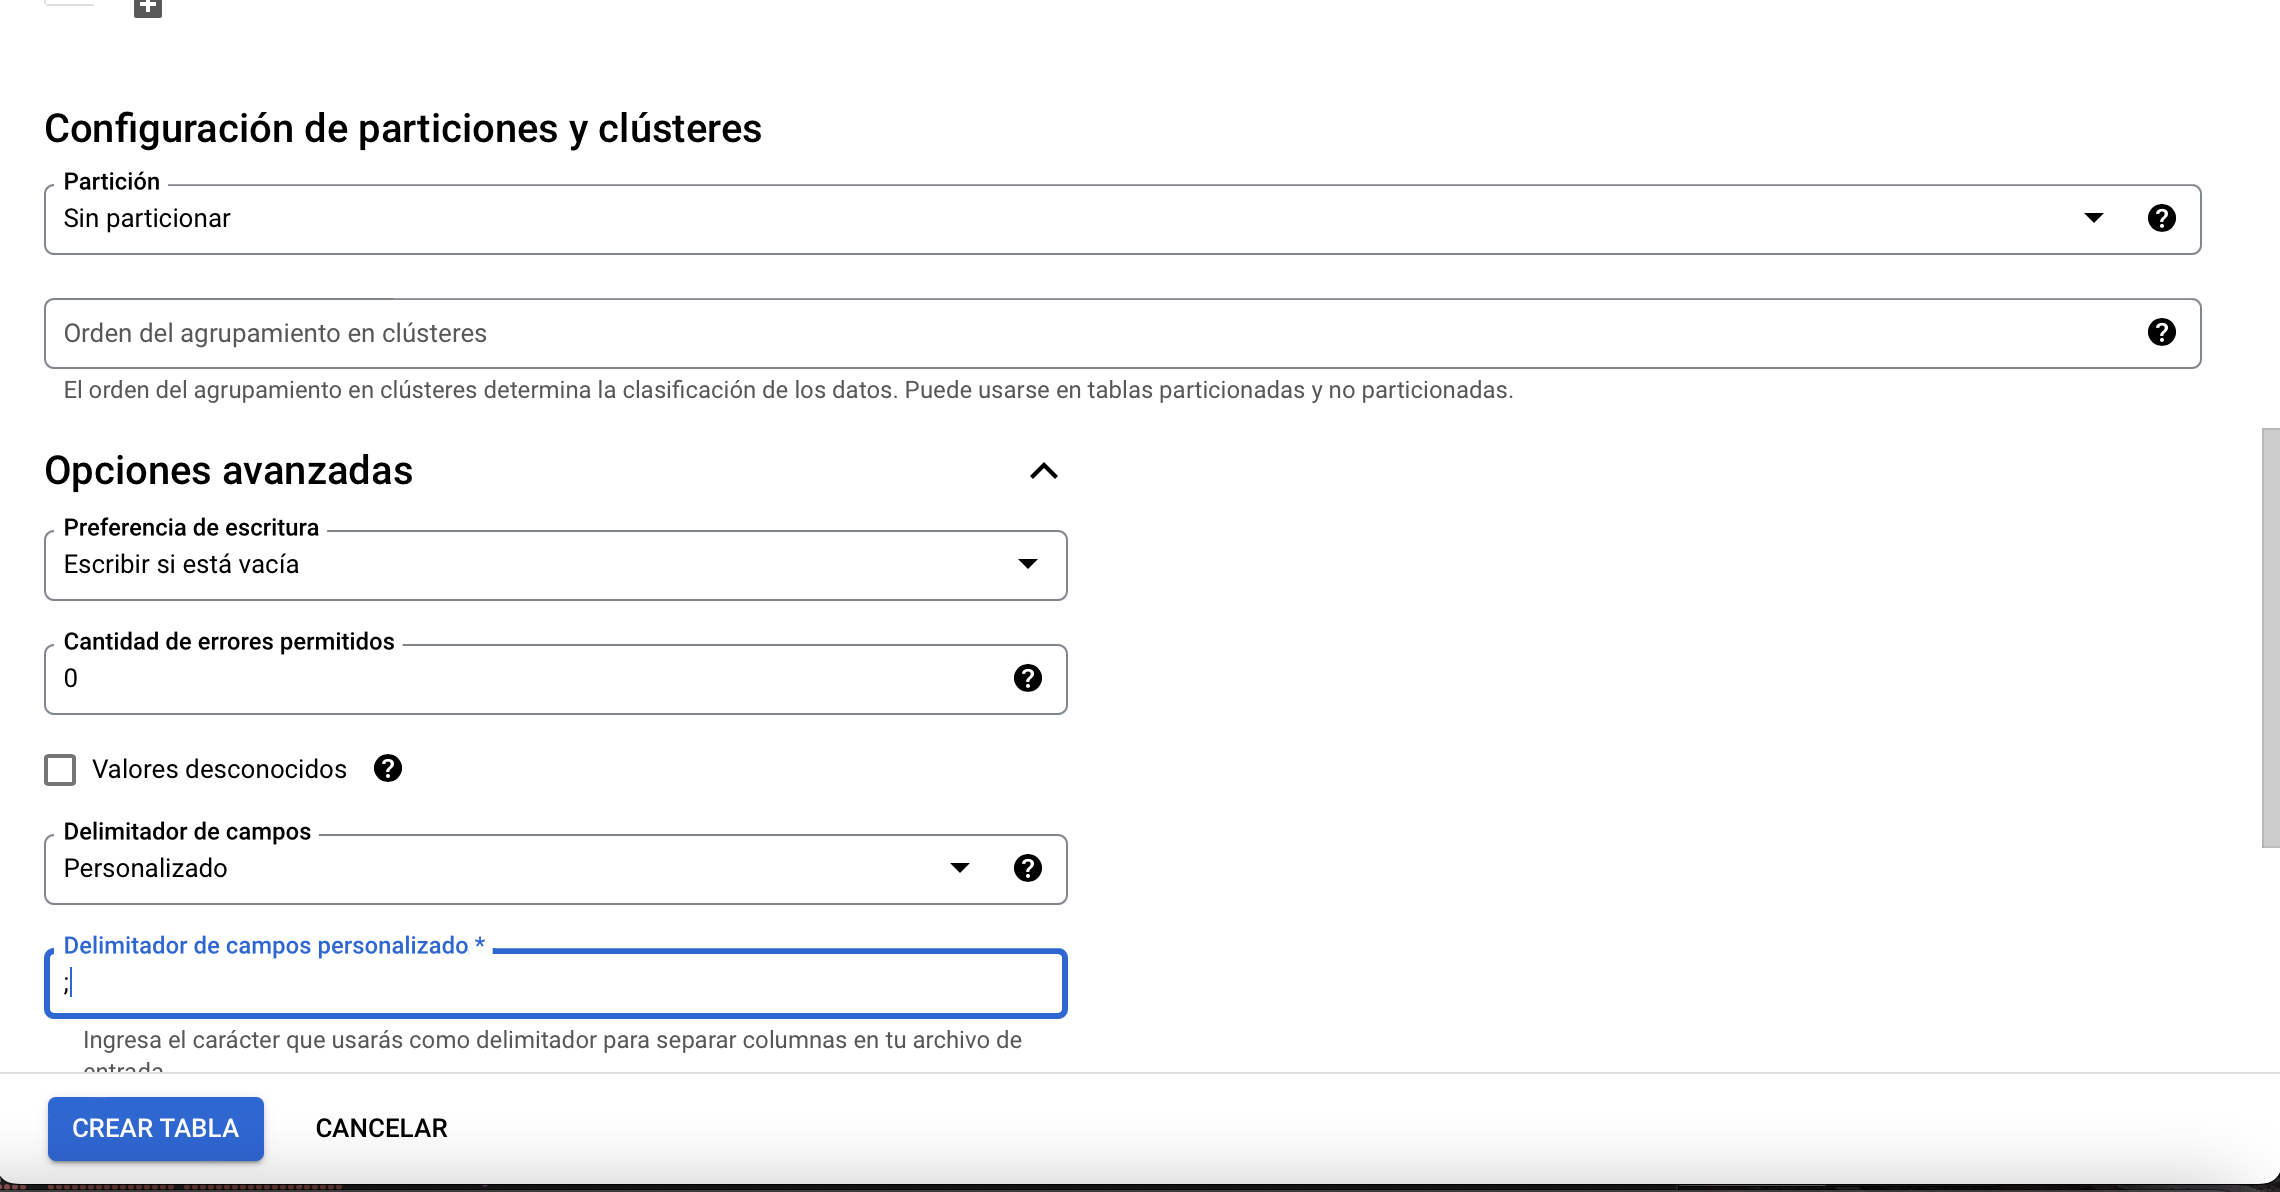
\includegraphics[width=7.25cm]{bq13}}%
\par

\caption{Lectura d'un arxiu extern}
\label{fig:bq12}
\end{figure}
\vspace{2mm}

Quant al projecte i al conjunt de dades, els deixarem com estan. I escollirem el nom de la taula, \verb|accidents_bd|, el qual farà saber que inclou informació sobre diversos accidents de trànsit. A continuació, tenim l'opció de definir explícitament l'esquema. No obstant això, atès que es tracta d'un arxiu CSV amb múltiples columnes, podem triar l'opció de detectar automàticament. D'aquesta manera, BigQuery donarà un cop d'ull al contingut de cada columna i determinarà quin ha de ser l'esquema. Més enllà d'això, al final de la finestra de creació de la taula ens apareixeran unes Opcions avançades. Aquestes opcions permeten la lectura de diferents tipus de CSV, entre d’altres coses. Sabem que el delimitador de camps d’un CSV pot ser una tabulació o una coma entre d’altres possibilitats. En el nostre cas, cal especificar que el nostre tabulador és el punt i coma “;”. 

\vspace{2mm}

Si hem establert totes aquestes especificacions, ja podrem començar amb l’anàlisi.

\vspace{2mm}

Ara es pot comprobar que \verb|accidents_bd| apareix sota el nostre conjunt de dades, \verb|dades_projecte|. A continuació, podem accedir a la informació de la taula i al seu contingut desplegant el menú i triant Obrir. En l'esquema de la taula, sabrà que s'ha detectat automàticament el tipus dels diferents camps. Donem un cop d'ull als detalls de la taula. Aquí notaràs que la grandària total és de poc més de 280 KB. El nombre de files és d'unes 2.780. I després, quan ens dirigim a la Vista Prèvia, obtenim un cop d'ull als continguts (Figura ~\ref{fig:bq13}). 

\vspace{2mm}
\begin{figure}[h!]
\par
\raisebox{-.5\height}{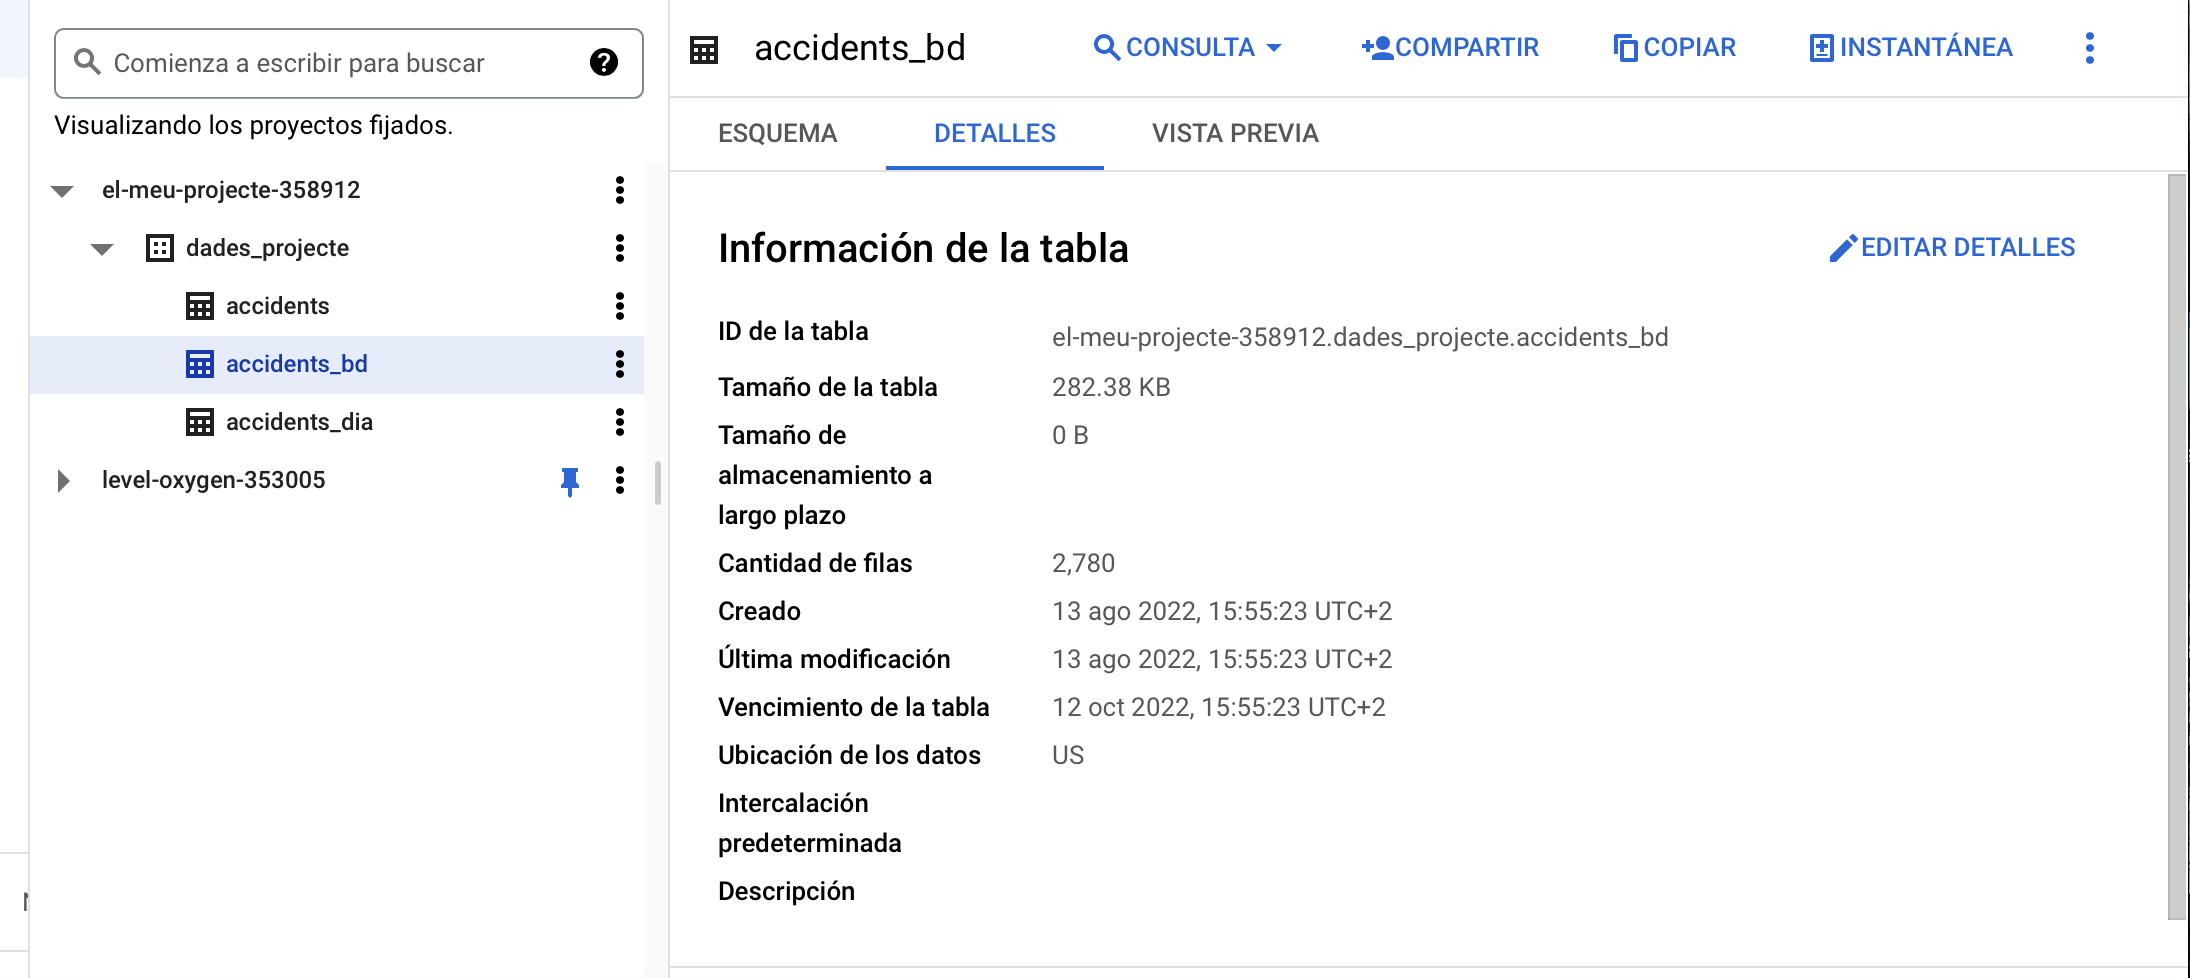
\includegraphics[width=7.25cm]{bq13_2}}%
\hfill
\raisebox{-.5\height}{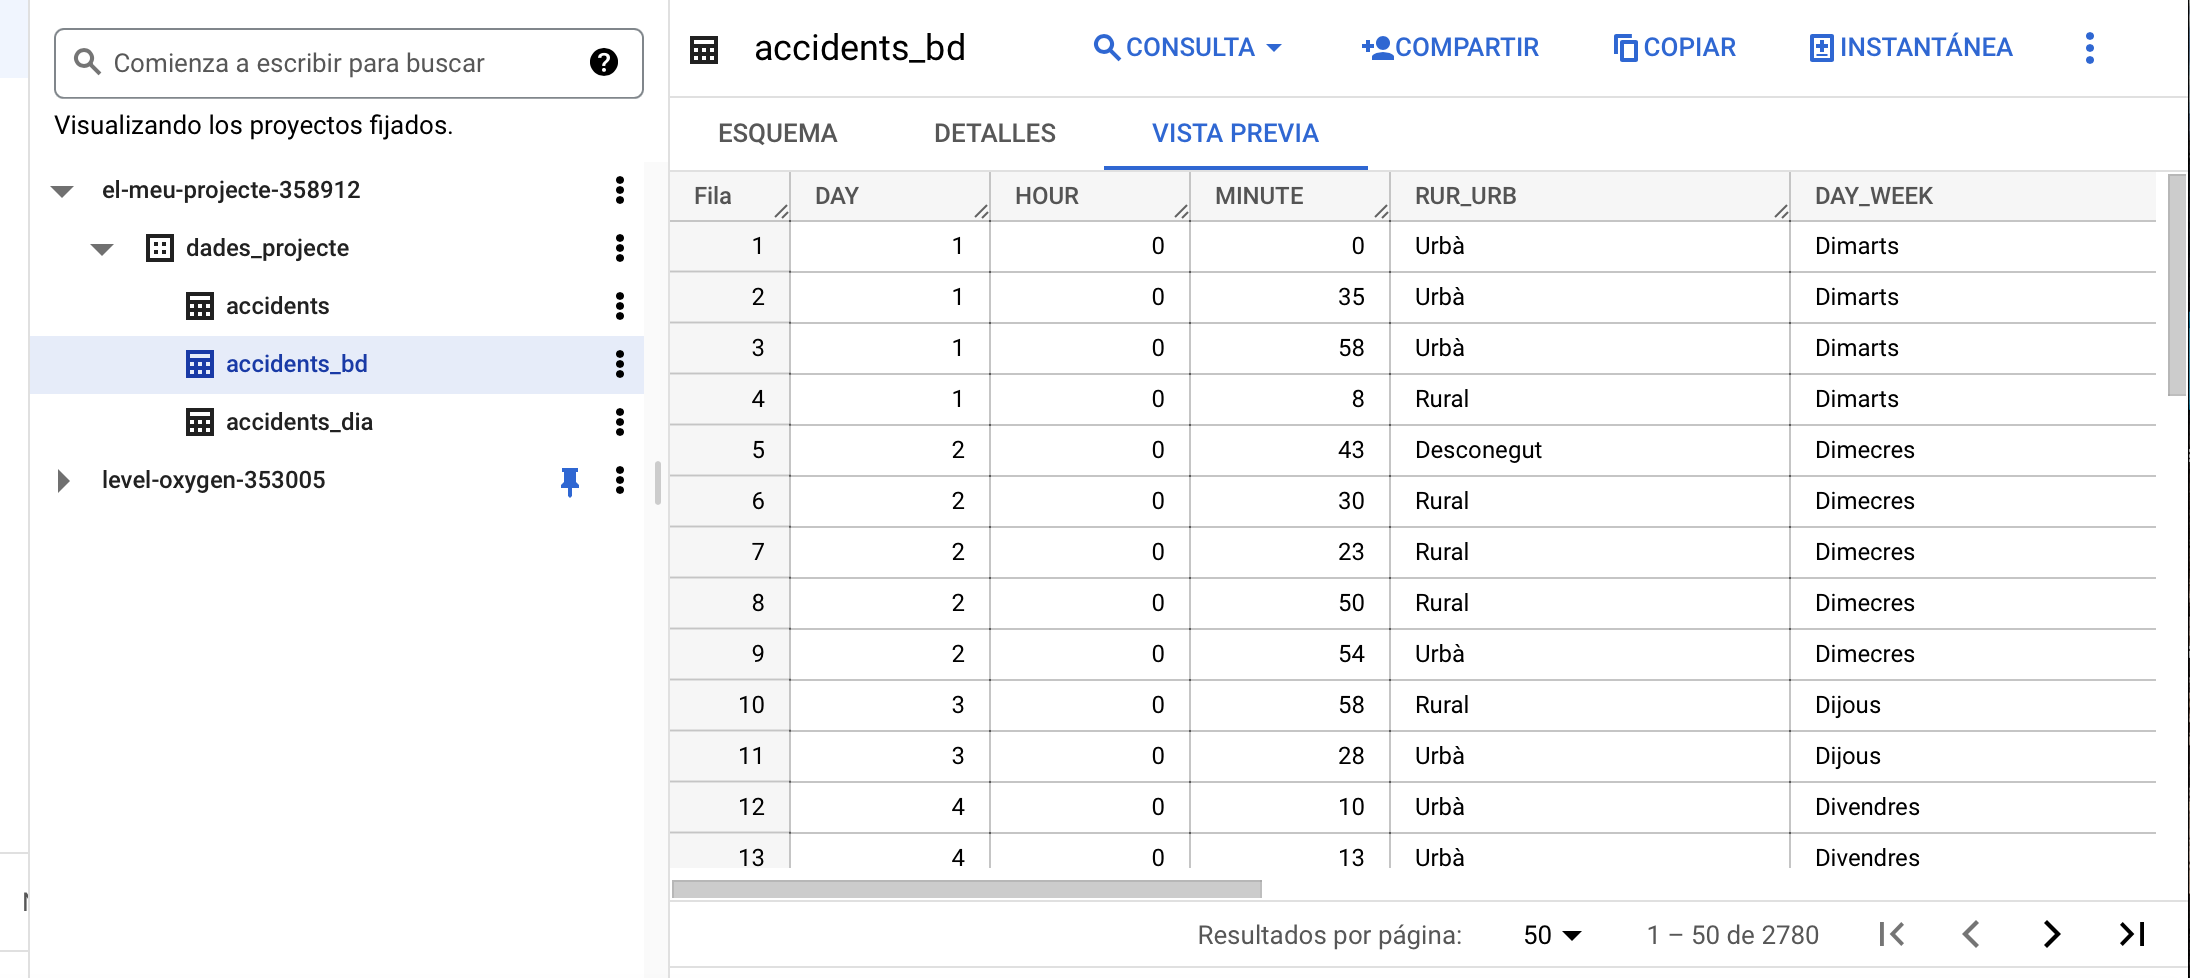
\includegraphics[width=7.25cm]{bq13_3}}%
\par

\caption{Informació sobre la taula}
\label{fig:bq13}
\end{figure}
\vspace{2mm}


\subsection{Consulta de dades i visualització d'estadístiques de consultes}

Ara, per a executar consultes en aquesta taula, ens dirigim al botó de consulta. Això ens permetrà obrir una nova pestanya de consulta. Aquesta pot ser una pestanya completament nova que ocultarà aquesta vista de detalls, mentre que una pestanya dividida ens permetrà fer referència a aquesta vista de detalls per a la taula mentre construïm una consulta. Observarà que ha aparegut una nova pestanya cap a la dreta, i que la consulta per defecte que apareix aquí inclou una clàusula SELECT però no hi ha camps després de SELECT. Precisament per això hi ha un error de sintaxi. Ara, per a completar la clàusula SELECT, podríem escriure els noms dels camps, o bé BigQuery inclou aquesta funció en la qual podem seleccionar els camps des de la vista de l'esquema. Per exemple, podem fer la consulta més bàsica a la base de dades, que ens retornarà la taula sencera:

\begin{verbatim}
SELECT *
FROM `[nom_projecte].[nom_base_de_dades].[nom_taula]`
LIMIT 1000
\end{verbatim}

\vspace{2mm}

Executarem aquesta consulta prement Executar. Els resultats han aparegut, i aquesta consulta s'ha executat en uns 0,3 segons per a mi. Per descomptat, podem desplaçar-nos i donar un cop d'ull a tots els resultats. No obstant això, el que és més interessant si ets nou en BigQuery són els detalls addicionals en el panell inferior. En concret, si ens dirigim a la secció d'Historial Personal, podem donar un cop d'ull als diferents treballs que s'han creat per a cada operació que hem realitzat. Per exemple, cada treball es classifica com QUERY si es realitza un SELECT o fins i tot un INSERT. Després es pot registrar una operació LLOEU per a quan carreguem les dades de l'arxiu CSV. Aquesta interfície sí que ens permet accedir a informació addicional per a cadascun dels treballs. Per exemple, si es mostren els detalls de l'últim treball creat, podem veure el que BigQuery ha fet per nosaltres per a assegurar-se que aquesta consulta s'executi i retorni els resultats. Aquí podem veure l'usuari que va iniciar aquest treball, quan es va crear exactament el treball, quan va començar i va acabar, i el més important, el nombre de bytes processats i el nombre de bytes facturats. Aquí podràs observar que el nombre de bytes facturats és de 10 megaoctets, que és de fet la quantitat mínima facturada per a cada consulta per Google Cloud Platform amb la finalitat de tenir en compte les despeses generals. Per a consultes més realistes que impliquin diversos megaoctets, o fins i tot gigaoctets, els bytes processats i els bytes facturats seran bastant similars. Sortint d'aquesta vista, passem a l'Historial del Projecte, que ens donarà els detalls dels treballs de tot el projecte i no sols del nostre propi usuari. I després està la secció de Consultes Guardades. Aquí és on es pot accedir a les consultes que hàgim guardat, encara que aquestes apareixeran en el menú de l'Explorador al costat dels nostres projectes i conjunts de dades.

\vspace{2mm}


Si escrivim a l’editor la nostra consulta, apareixerà un validador d’aquesta a la part superior dreta de la finestra. Aquest validador pot agafar dues formes:
- Si la consulta és vàlida, apareixerà un icona de verificación verd.
- Si la consulta no és vàlida, aparaixerà un icona d’exclamació Vermell
A més, el validador també mostra la quantitat de dades que la consulta processarà quan s’executi. Per exemple, si demanem en una consulta que ens retorni una columna selncera, el validador de la dreta ens marca que es processaran una quantitat de gairebé 22KB, tal i com es pot veure a la figura ~\ref{fig_bq16}.

\vspace{2mm}
\begin{figure}[h!]
\begin{center}
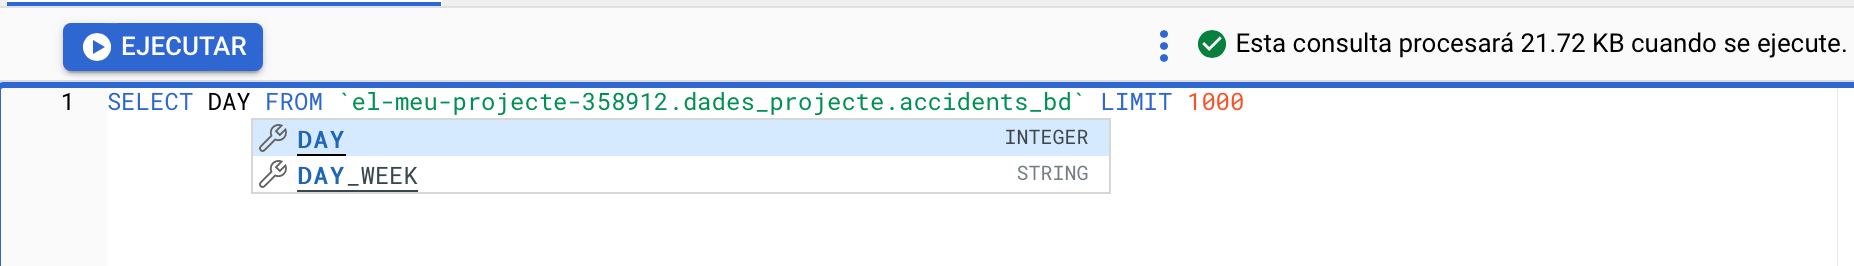
\includegraphics[width=10cm]{bq16}
\end{center}
\caption{Exemple del funcionament del validador de consultes}
\label{fig:bq16}
\end{figure}
\vspace{2mm}

\subsection{Creació d'una taula a partir d'un resultat de consulta}

Després d'haver introduït dades de fonts externes en BigQuery. Ara veurem com podem crear noves taules a partir de les existents. En concret, la taula en l'Editor de Consultes. Ara he inserit una consulta que selecciona una sèrie de camps diferents, incloent-hi el nom, la companyia, el gènere i el director de la taula en el conjunt de dades. Es tracta de pel·lícules el pressupost de les quals és superior a 100 milions de dòlars. L'objectiu és crear una nova taula a partir dels resultats d'aquesta consulta concreta. Aquí apliquem un filtre, no sols eliminant els rols a causa de la clàusula where i seleccionant només camps específics. Però vostè notarà en línia número dos que també creguem una nova columna anomenada benefici, que es computa mitjançant el càlcul de la diferència entre el creixement de les pel·lícules. És a dir, la quantitat de diners que va ingressar i després restant el pressupost d'aquesta. Per descomptat, per a veure el cost associat a aquesta consulta. Podem minimitzar l'Explorador. I ara sabem que encara que el cost calculat apareix com 492 kilobytes en aquest cas. El cost real serà de 10 megaoctets que és el mínim per a BigQuery. Quan executem això, els resultats apareixen i hi ha un total de 315 files de dades. Ara hem d'exportar totes aquestes dades a una nova taula. Revisa algunes de les opcions d'exportació. Podem donar un cop d'ull al menú Guardar resultats. Vostè observarà que hi ha un nombre de diferents opcions aquí per a la manera de guardar els resultats. Podem guardar-los com un arxiu CSV en Google Drive o en un arxiu local. El format JSON també està disponible com una opció d'exportació. No obstant això, el que oferirem aquí és exportar el contingut a una nova taula de BigQuery. Una vegada feta aquesta selecció, podem decidir el nom del projecte i el conjunt de dades on s'aprovisionarà la taula i després establir un nom de taula. La cridaré simplement. Llavors, quan guardem les coses, això haurà iniciat un nou treball per a aprovisionar la nova taula i carregar-la amb dades. Una vegada que tanquem aquesta notificació, podem treure el pin de l'Explorador i baix, apareix com una taula. En obrir-la confirmem que l'esquema apunta a les mateixes columnes que havíem referenciat en la clàusula select de la consulta que va crear aquesta taula, encara que hi ha una columna anomenada profit el tipus de la qual s'ha establert com un enter. Des dels detalls podem confirmar que el nombre de files coincideix amb el dels resultats de la consulta, concretament 315. I després la vista prèvia ens mostrarà quins són exactament les dades. Desplacem-nos i confirmem que la columna de beneficis es deriva, efectivament, del creixement i del pressupost. Quin és llavors la finalitat d'aquesta taula? Bé, atès que només conté un subconjunt de la taula original. Significa que les consultes contra això tindran potencialment menys dades per a processar que les consultes que s'executen directament contra. Si només volem analitzar les pel·lícules de gran pressupost amb un pressupost de més de 100 milions, és millor executar les nostres consultes en aquesta taula més petita, que inclou tota la informació que necessitem i probablement tindrà un cost de consulta menor. Per a executar una consulta d'aquest tipus, obrirem l'Editor de Consultes i a substituir aquesta consulta directament contra per aquesta altra que es dirigeix a la taula recentment creada. Observarà que els camps de la clàusula select són idèntics als quals teníem anteriorment, però la clàusula where és una mica diferent. I mentre que la consulta anterior va processar 492 kilobytes, aquesta només funcionarà amb 34,7. Seguim endavant i executem aquesta consulta. I els resultats confirmen que les consultes contra aquesta taula funcionen com s'espera que ho facin.

sèrie temporal de 31 observacions, on per cada dia digui el nombre d’accidents ocorreguts amb víctimes.

\begin{verbatim}
SELECT DAY, COUNT(*) AS FREQ
FROM `level-oxygen-353005.examen_final.accident`
GROUP BY DAY
\end{verbatim}

\vspace{2mm}
\begin{figure}[h!]
\par
\raisebox{-.5\height}{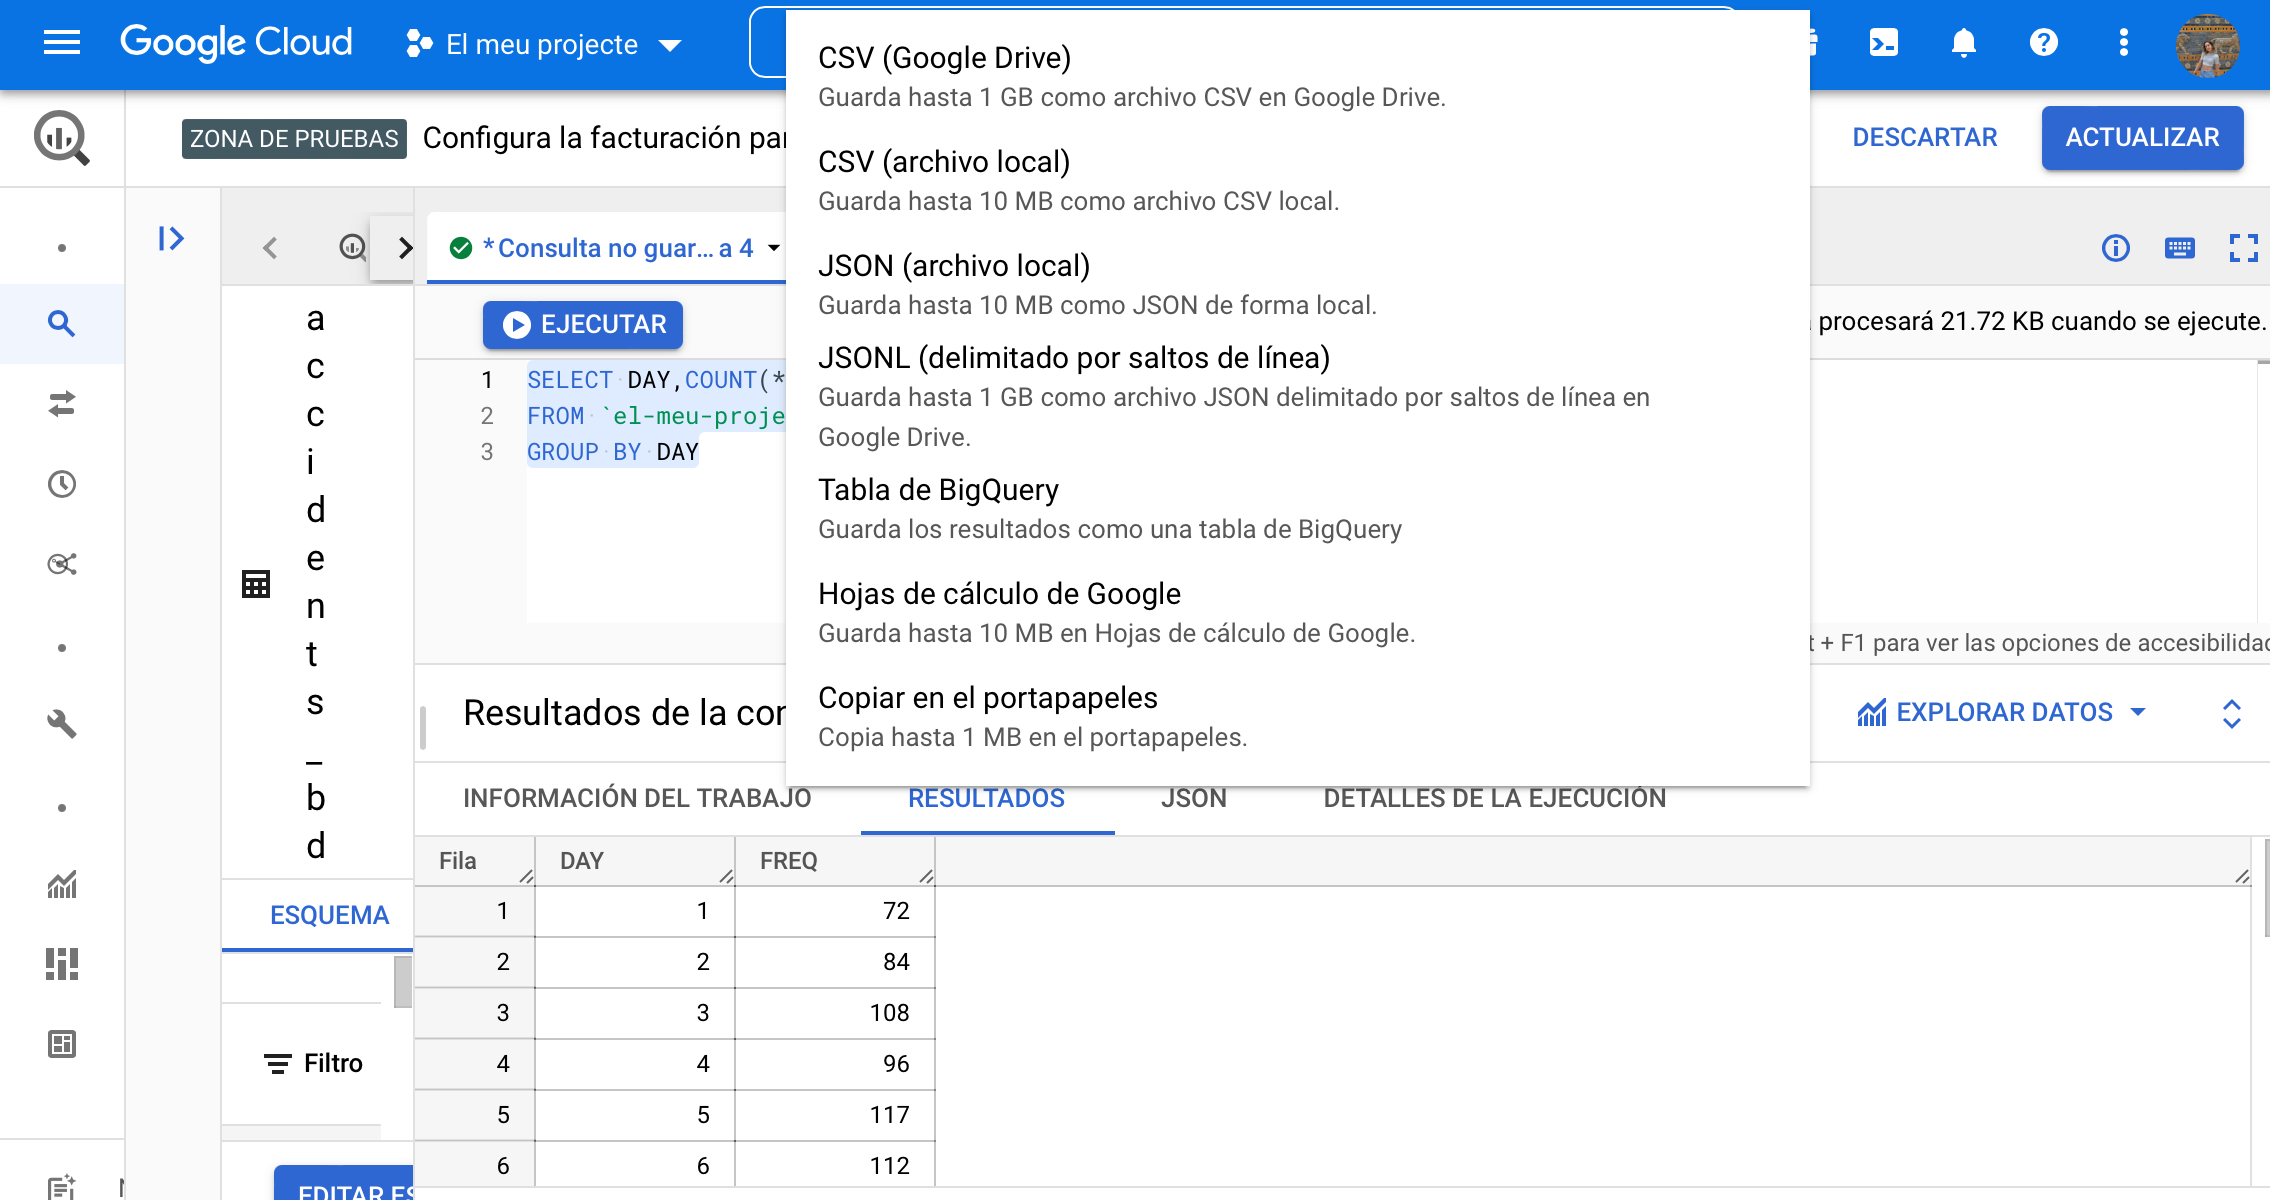
\includegraphics[width=7.25cm]{bq17}}%
\hfill
\raisebox{-.5\height}{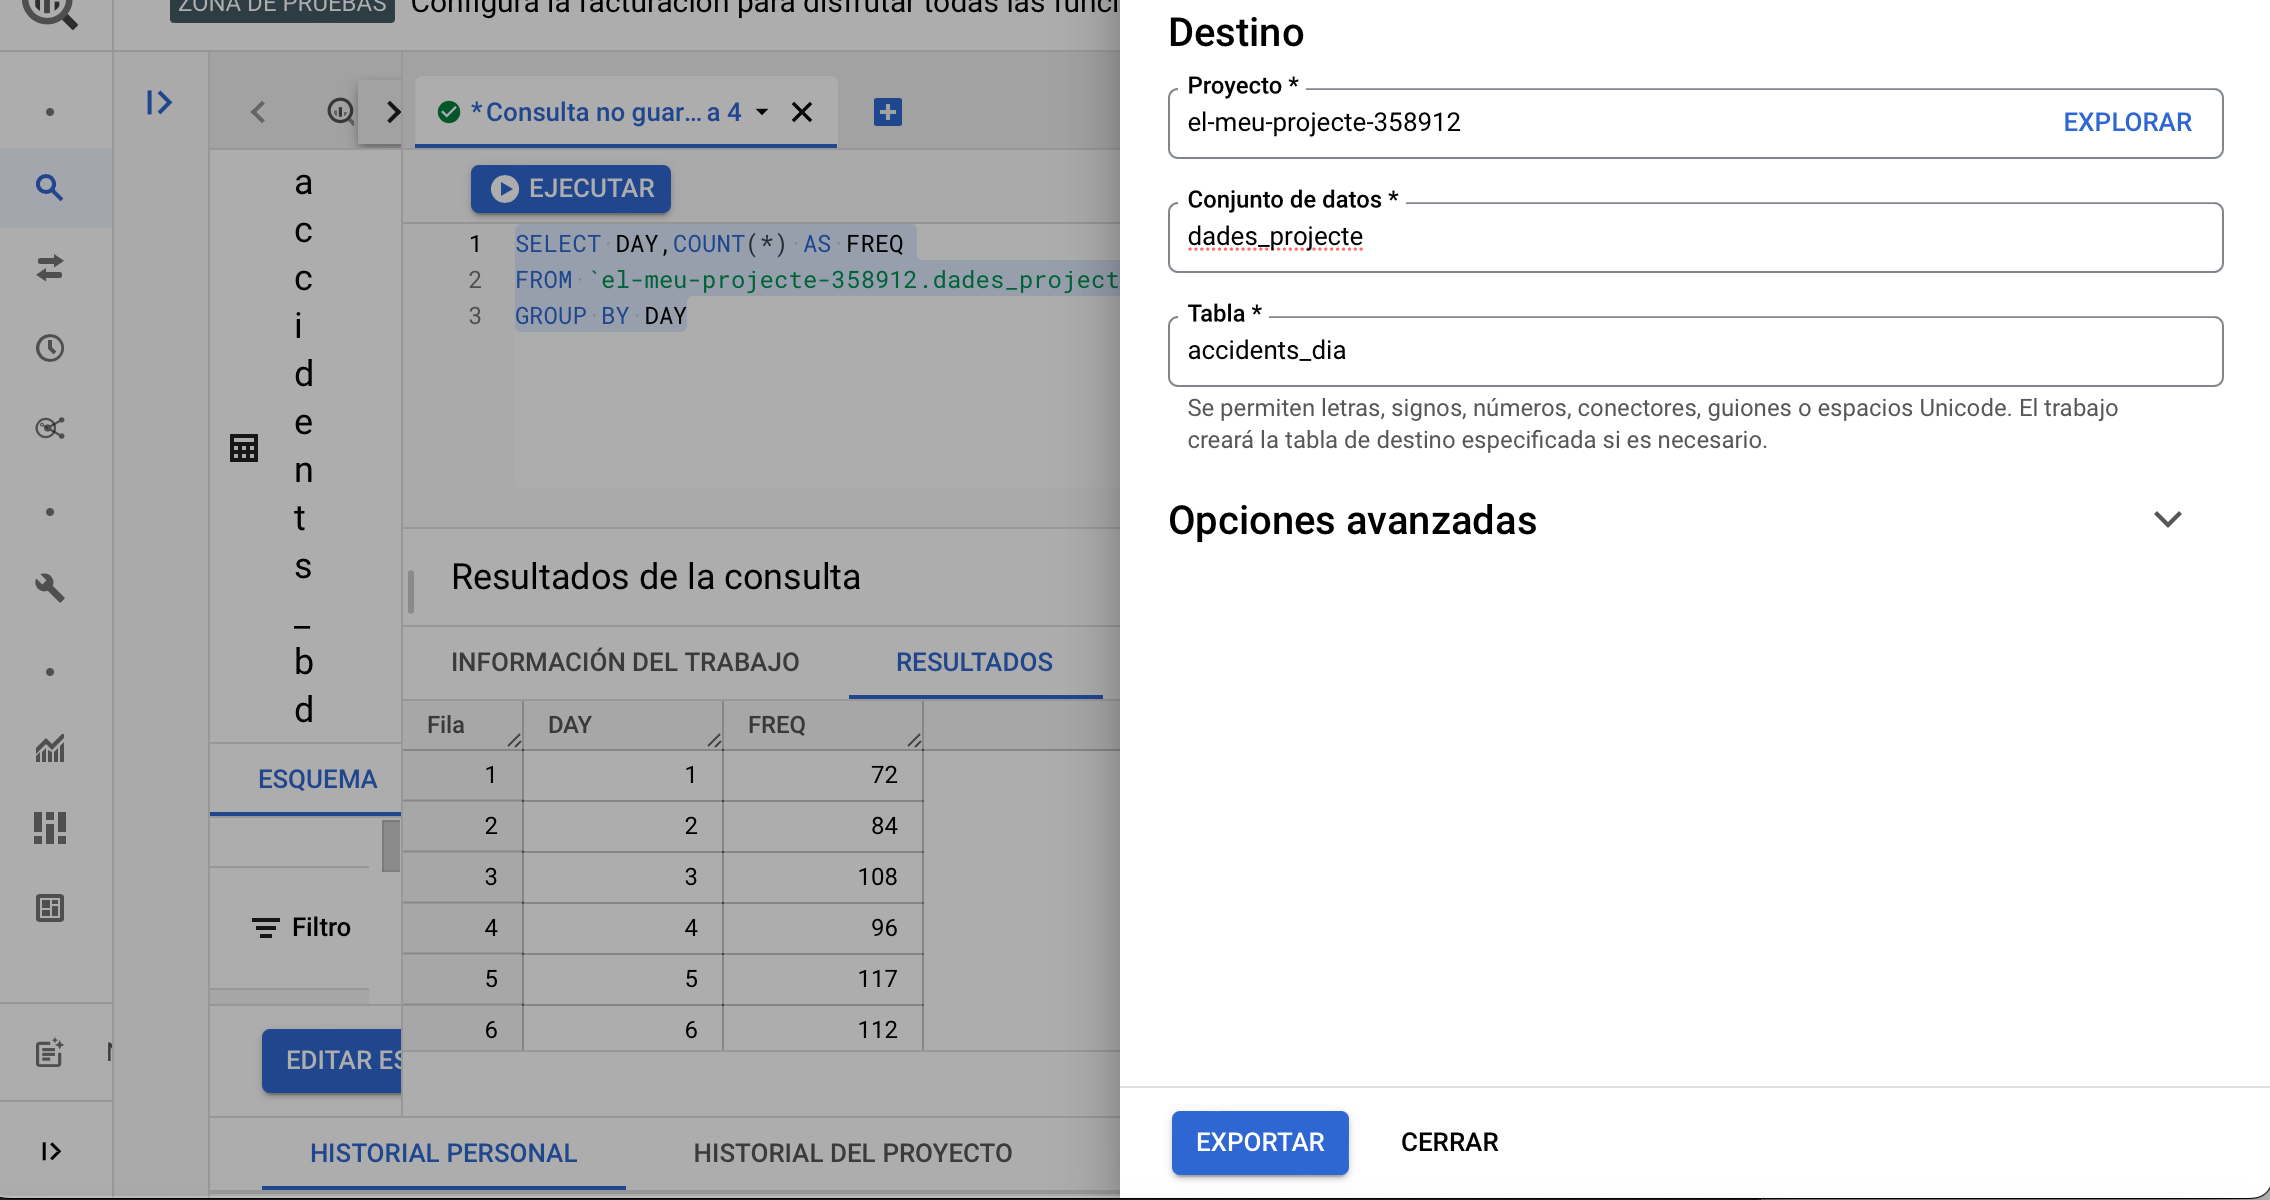
\includegraphics[width=7.25cm]{bq18}}%
\par

\caption{Creació d'una taula a partir d'una consulta}
\label{fig:bq17}
\end{figure}
\vspace{2mm}


\newpage

\section{Execució de consultes i visualització de resultats}

\subsection{Conjunts de dades públics a BigQuery}

Mentre es familiaritza amb BigQuery, li serà útil fer ús d'alguns dels conjunts de dades disponibles públicament per a executar consultes i simplement acostumar-se al servei i les seves diverses característiques. Aquests conjunts de dades públiques es troben en un projecte anomenat BigQuery Public Data. Per a arribar a ells, utilitzem la funció de cerca del panell de l'Explorador. Tingues en compte que podem ampliar la nostra cerca per a incloure tots els projectes d'accés públic i BigQuery Public Data hauria d'aparèixer en els resultats. Pot donar un cop d'ull als diferents conjunts de dades i taules d'aquest projecte. Però si faràs referència a ell periòdicament, t'ajudarà ancorar-ho perquè sigui fàcilment accessible en el panell de l'Explorador. Ara treballarem amb un conjunt de dades i una taula específics dins d'aquest projecte. Per a això, deixa'm netejar una mica les coses en aquesta vista de l'Explorador. I després, dins del projecte de dades públiques de BigQuery, haurem de navegar fins a un conjunt de dades específic que conté informació sobre la població mundial recopilada pel Banc Mundial. És possible que hàgim d'ampliar els resultats primer. I després, en desplaçar-nos cap a la part inferior, trobarem el conjunt de dades de població mundial del Banc Mundial. Dins d'aquest, hi ha una taula anomenada població per país. Aquesta, per descomptat, és només una de les taules que estan disponibles en aquest projecte i que podem utilitzar per a familiaritzar-nos amb BigQuery. Abans d'iniciar qualsevol consulta, l'obrirem per a poder veure la seva informació i fer-nos una idea de les dades que conté. En l'esquema, podem veure que hi ha una columna de país i després tenim diverses columnes que assenyalen la població del país en diferents moments. A continuació, passem a la pestanya Detalls, on observem que aquesta taula és bastant petita, amb només uns 125 kilobytes i 264 files. També observarà que aquesta taula està particionada. Així que les seves dades es dividiran en diversos nodes. I aquesta partició es basarà en el temps d'injecció. Això està implícit en la propietat Partitioned on Field que té un valor de temps de partició, que és de fet una pseudo-columna i que no veurem en l'esquema d'aquesta taula. Passem llavors a la vista prèvia. Aquí, veiem que hi ha una columna de país al costat d'un codi de país, i després desplaçant-nos, observem que els valors de població per a la majoria dels anys inicials no són presents per a unes certes files, però les dades particionados estan disponibles per als anys més recents. Tornant enrere, podem veure que aquesta taula inclou no sols la població de diversos països, sinó també diversos grups de països. Per exemple, aquí hi ha un grup anomenat Europa i Àsia Central.

\subsection{Configuració i ús de memòria cau de BigQuery}

Ara estem en condicions de consultar la taula pública a la qual acabem d'accedir, i mentre ho fem, també explorarem com BigQuery emmagatzema en caixet els resultats de la consulta perquè les dades puguin ser recuperats més ràpidament la pròxima vegada que s'executi la consulta. En primer lloc, dona un cop d'ull a la consulta que acabo de pegar en l'Editor de Consultes. En primer lloc, cridaré la seva atenció sobre la clàusula frontal en la qual fem referència a la taula de població per països, especificant la seva part completa, començant pel nom del projecte, BigQuery Public Data. Després el nom del conjunt de dades, World Bank Global Population, i només llavors especifiquem el nom de la taula. Els camps que projectem en els resultats de la consulta inclouran el país, el codi de país, juntament amb les poblacions en 1960 i 2018. També projectem la diferència de poblacions entre aquests dos anys com un canvi absolut. També ordenarem els resultats en l'ordre descendent d'aquest valor de canvi absolut. En continuar i executar aquesta consulta, observarem que la consulta es va completar en tot just 0,3 segons per a mi, i es va processar un total de 9,1 kilobytes. Podem confirmar que això ens retorna un total de 264 files, és a dir, totes les files del conjunt de dades. El que aquesta sortida no ens diu és que, sota el capó, BigQuery ha emmagatzemat en caixet aquests resultats de la consulta, tots els 9,1 kilobytes, de manera que quan executem la mateixa consulta una vegada més, els resultats s'obtindran de la caixet en lloc d'en el disc. Podem comprovar-ho simplement tornant a executar la mateixa consulta. En aquesta execució, observarà que el temps de finalització de la consulta s'ha marcat com zero segons, i podem veure explícitament aquí que els resultats s'han recuperat de la caixet. També pot confirmar que s'han retornat les mateixes 264 files de dades. No obstant això, cal tenir en compte que només s'accedeix a les dades de la caixet quan s'executa la mateixa consulta després de la seva creació. Per exemple, si es modifiqués una mica aquesta consulta, per exemple, aquí només he canviat la clàusula select, i això inclou els camps de país i canvi absolut que es van recuperar en la consulta anterior i s'han emmagatzemat en la caixet. En altres paraules, els resultats de la consulta d'aquesta execució haurien de retornar-nos un subconjunt de les dades que ja són presents en la caixet. No obstant això, per la forma en què funcionen les caixets de BigQuery, quan executem això, observarem que l'execució de la consulta m'ha portat 0,4 segons, i que la informació no s'ha recuperat de la caixet. No obstant això, quan aquesta consulta es torna a executar, és quan la caixet s'activa, i és d'on es recuperen les dades. Per tant, la caixet només funciona si és la mateixa consulta la que es reexecuta. Fins i tot un subconjunt dels resultats de la consulta no pot ser recuperat de la caixet. Si vols desactivar la caixet, podem expandir les opcions aquí, i després anar a la Configuració de la Consulta on pots desplaçar-te a les preferències de la caixet, i després desmarcar aquesta casella per a usar els resultats de la caixet. Permetin-me seguir endavant i fer això. Una vegada que aquesta casella estigui desmarcada, però abans que diguem les coses, trauré la informació original per a l'emmagatzematge en caixet, on observarà que si les dades resideixen en la caixet, també significa que no se'ns facturarà per cap visita a la caixet. Així que l'emmagatzematge en caixet és una gran manera de reduir el cost d'execució de les consultes, i per descomptat també millora el rendiment d'aquestes. No obstant això, si vostè sent que la caixet pot ser encara, ja que aquestes dades es manté sense canvis durant 24 hores, així, és possible que desitgi desactivar com ho hem fet aquí. Llavors, quan diguem que les coses baixen i seguim endavant i tornem a executar la mateixa consulta, aquesta vegada, els resultats s'han obtingut del disc i no de la caixet. Per si de cas, pots continuar executant aquesta consulta tantes vegades com vulguis. I en cada execució, observaràs que el temps de processament és superior a zero segons i que no s'ha accedit a la caixet.

\subsection{Taules externes de BigQuery}

En aquesta demostració, crearem una taula externa en BigQuery extraient les dades d'un full de càlcul de Google abans de consultar-la i després visualitzar les seves dades. En primer lloc, veuràs que he tret un full de càlcul de Google buida, que emplenaré amb el contingut d'un arxiu d'Excel en el meu propi sistema d'arxius. Pots seguir-me tirant d'un full de càlcul, i després dirigir-te a Importar, i triar l'opció de carregar des del sistema d'arxius. Podem arrossegar i deixar anar aquí, o prémer aquest botó, i després navegar a aquest arxiu de Honey Production. Això s'inclou en els materials del curs, però també podria ser descarregat com un arxiu CSV d'aquesta ubicació en Kaggle.com abans de convertir a Excel. A continuació, introdueixi les dades de la Producció de mel en el full de càlcul de Google. Haurà de subministrar algunes confirmacions aquí, però aviat es carreguen les dades. Observaràs que això inclou diverses estadístiques sobre la producció de mel per a diferents estats dels Estats Units. Aquest full de càlcul també inclou una fila de capçalera. Analitzarem aquestes dades una vegada que els introduïm en BigQuery, però per a arribar a aquest pas, primer canviarem el nom d'aquest full de càlcul per un altre una mica més representatiu. Després, per a accedir a aquest full de càlcul des de BigQuery, necessitarem aquesta URL, així que copiem això i després canviem a BigQuery. Aquí, crearem una nova taula sota el conjunt de dades una vegada més. En aquesta ocasió, la font de les nostres dades serà Google Drive. Això també significa que haurem d'especificar un URI a les dades de Google Drive. Simplement pegaré l'enllaç al full de càlcul que acabem de copiar, i atès que l'arxiu de Google Drive podria ser realment qualsevol cosa, haurem d'establir explícitament el format d'arxiu a Google Sheet en aquest cas. A continuació, deixarem el projecte i el conjunt de dades com estan, i el nom de la taula pot ser. Observarem que el tipus de taula s'ha establert automàticament com a taula externa, cosa que significa que les dades residiran fora de BigQuery, és a dir, en Google Drive. Podem configurar l'esquema perquè sigui autodetectat, i hi ha un altre canvi de configuració que haurem de fer. Atès que el nostre full de càlcul té una fila de capçalera, podem ampliar les opcions avançades, i després establir el nombre de files de capçalera per a saltar com un. Amb aquestes especificacions, seguim endavant i creem aquesta taula a partir d'un full de càlcul de Google, i observaràs que apareix sota el conjunt de dades. Per a fer-nos una idea de com està estructurada aquesta taula, l'obrim. Aquí, en l'esquema de la taula, notaràs que el tipus de les diferents columnes sembla haver estat configurat correctament, on l'any és un enter, i també apareixen diversos valors de punt flotant. Després, quan ens dirigim als detalls, aquí és on veiem una cosa interessant. La grandària de la taula aquí és de zero bytes, atès que les dades són de fet externs a BigQuery. Si ens desplacem, podem veure els detalls de les dades externes. Això significa que quan actualitzem el full de càlcul, qualsevol consulta contra aquesta taula recollirà automàticament les dades més recents. Ja que la nostra consulta de la taula gran no és només una còpia del full de càlcul, sinó que és de fet una referència a ella. Parlant de consultar les dades, ens dirigirem a Query, i a obrir un editor de consultes en una nova pestanya. Començaré amb una consulta molt simple, seleccionar estrella d'aquesta taula. Quan aquesta consulta s'executa, totes les dades són retornats a nosaltres, i podem accedir a ells com ho faríem amb qualsevol dada que resideixi en una taula nativa de BigQuery. Ara ja sabem com funcionen les taules externes en BigQuery.

\subsection{Integració de BigQuery amb Data Studio}

Ara que hem cobert els diferents tipus de taules de BigQuery. Ens centrarem en com podem analitzar-les utilitzant visualitzacions. Ja tenim aquí els resultats d'una consulta SELECT. I per a realitzar una anàlisi addicional de les dades, podem ampliar el menú Explorar dades. Aquí observarem que l'única opció present és la d'explorar les dades mitjançant Data Studio, que és el servei de visualització de Google Cloud Platform. Quan fem aquesta selecció, notaràs que ha sorgit una interfície, que ja té una taula que conté alguna informació agregada. Tenim el camp d'estat juntament amb un recompte de registres que indica el nombre d'ocurrències d'un valor específic en la columna d'estat. No obstant això, per a la nostra visualització, és un tipus d'agregació diferent el que necessitarem en lloc d'un recompte de registres per a diferents valors d'estat. Primer, no obstant això, seleccionarem una visualització abans de configurar-la per a presentar la informació que necessitem. Des del menú de la dreta, podem començar amb un simple gràfic de barres. Observarà que aquest ja presenta la informació agregada que és present en la taula. Ara, per a reconfigurar aquest gràfic de barres, minimitzarem el menú del gràfic, i això ens farà veure la configuració del gràfic. Aquí sabrà que hi ha una propietat de dimensió i que aquesta apunta al camp que s'utilitzarà per a agrupar les dades. Així que per defecte, s'ha realitzat una agrupació per la columna d'estat. Seguirem amb això. Tanmateix, el que canviarem és la mètrica d'agregació. Per defecte s'ha establert el recompte de registres. No obstant això, agregarem en el seu lloc el valor de la producció de mel per a cada estat. Podem arrossegar i deixar anar prodvalue a la propietat mètrica, i després ens desfarem d'aquesta mètrica de recompte de registres. I aquí ho tenim. Tenim la producció de mel en termes de valor de producció per a cada estat basat en el nostre conjunt de dades. I això ens diu clarament que els estats de Dakota del Nord i Dakota del Sud van ser els més productius. Ara, per defecte, és una suma del valor de la producció que s'ha calculat. Si vols canviar el tipus d'agregació, pots simplement editar això. I això ens presenta funcions d'agregació com a mitjana, comptatge, mínim, etc. Ens quedarem amb la suma aquí. Després podem desplaçar-nos per a veure altres propietats de configuració, però ara com ara, ens quedarem amb aquest gràfic de barres com està. Després podem canviar el nom d'aquesta pestanya particular en la visualització. Li donaré un nom representatiu de prodvalor per estat. Més enllà d'això, també podem establir un nom per a tota la visualització. Cridaré a aquesta mel de producció, i després premi guardar. I una vegada guardat aquest informe, podem seguir endavant i afegir una segona pestanya en la qual inclourem un gràfic diferent. Per al gràfic, ampliarem el menú de gràfics. Aquesta vegada inclourem un gràfic de sèries temporals suavitzades. Observarem que, per defecte, és la columna de l'any la que apareix en l'eix X, i és el valor de la producció de mel el que apareix en l'eix I. No obstant això, hi ha una línia separada per a cada estat. Si observa la configuració del gràfic, observarà que és la columna de l'any la que apareix com a dimensió principal, però també hi ha una columna de desglossament que apunta a l'estat. Això significa que sota el capó s'ha realitzat una operació d'agrupació per basada en els camps d'any i estat. A més, tingui en compte que les visualitzacions generades en Data Studio són interactives. Es pot obtenir informació addicional passant el ratolí per sobre de diferents punts del gràfic. No obstant això, mantinguem aquest gràfic simple i eliminem aquest camp de desglossament, la qual cosa ens dona un gràfic més simple i menys sorollós. Amb aquesta nova pestanya en el seu lloc, repetirem els passos que realitzem anteriorment establint un nou nom per a aquesta pestanya. La diré Valor de producció total en el temps. Assegura't que aquest gràfic s'ha guardat amb els canvis. I ara en cas que t'estiguis preguntant com pots accedir a aquesta visualització. Bé, pots copiar aquesta URL datastudio.google.com per a accedir a aquest servei. Navegaré a aquest enllaç en una nova pestanya. Això farà que aparegui el teu propi panell de control de Data Studio en el qual pots navegar a l'Explorador. I si els continguts estan ordenats en ordre descendent de temps, Producció de Mel hauria d'aparèixer en la part superior aquí. Quan es fa clic en això, és la mateixa visualització en la qual acabem de treballar. Per descomptat, podem confirmar-ho accedint a la segona pestanya. Efectivament, apareix el gràfic de sèries temporals. Cal tenir en compte que també podem compartir aquest informe amb altres usuaris. Amb això hem completat un ràpid cop d'ull a Data Studio i la seva integració amb BigQuery.

\newpage

\listoffigures


\end{document}
